\documentclass[a4paper,12pt, titlepage]{article} 
\usepackage{geometry}           % пакет для задания полей страницы командой \geometry
\geometry{left=3cm,right=1.5cm,top=2cm,bottom=2cm}
\usepackage[utf8]{inputenc}
\usepackage[english,russian]{babel}
\usepackage{amsmath}
%\usepackage{amsthm}
%\usepackage{cmap}
\usepackage{indentfirst}
\usepackage{a4wide,amssymb}
%\usepackage[pdftex]{graphicx}
%\usepackage[pdftex]{graphics}
%\usepackage{wrapfig}
%\linespread{1.3}                % полтора интервала. Если 1.6, то два интервала
\pagestyle{plain}               % номерует страницы

\usepackage{graphicx}
\renewcommand{\topfraction}{1}
\renewcommand{\textfraction}{0}

%opening
%\title{План дипломной работы\\
%Коррекция многогранников с помощью локальных деформаций}
%\author{Палачев Илья, 510 группа}

\begin{document}

\begin{titlepage}
\begin{center}
Московский государственный университет им. М. В. Ломоносова\\

Механико-математический факультет\\
Кафедра вычислительной математики\\
\end{center}

\vspace{5cm}

\begin{center}
\LARGE \bf{Коррекция многогранников с помощью локальных деформаций}
\end{center}

\begin{center}\large
Диплом
\end{center}

\vspace{3cm}

\large
\begin{flushright}
\textbf{Выполнил:}\\
студент группы 510\\
Палачев Илья Александрович\\

\vspace{1cm}


\end{flushright}

\vspace{1cm}

\begin{center}
Москва 2012
\end{center}

\end{titlepage}

%\maketitle
\tableofcontents
%\begin{abstract}
%\end{abstract}

\newpage
\section{Введение}
\subsection{Происхождение вопроса}
\begin{flushleft}
Данная работа возникла из вопроса автоматизации производственного процесса огранки драгоценных 
камней. 
\end{flushleft}
\begin{flushleft}
Огранка подразумевает создание на поверхности камня ряда геометрически правильных плоскостей, 
граней, от которых будет отражаться попадающий внутрь кристалла свет. После многократного 
внутреннего отражения и преломления лучи света разделяются на спектральные составляющие и, 
покидая камень, создают игру оттенков на его поверхности.
Огранка различается по сложности выполнения. В наиболее сложной и привлекательной бриллиантовой 
огранке может быть до 240 граней. Простая огранка создает на поверхности камня 30 плоскостей.
Качественно выполненная огранка существенно повышает стоимость драгоценного камня, в то же 
время неправильная огранка может «убить» камень, внести в него дефекты \cite{wiki-ogranka}. 
\end{flushleft}
\begin{flushleft}
В конечном счете красота бриллианта определяется оптическими свойствами, как присущими 
веществу - алмазу, так и проявляющимися в результате огранки и полировки. Совокупность 
поверхностных и внутренних оптических свойств бриллианта человеческий глаз воспринимает 
как попавшие в глаз разнообразные лучи — белые и цветные, в целом создающие картину 
бриллианта \cite{3dbook}. 
\end{flushleft}
\begin{flushleft}
 Форма огранки бриллианта зависит от формы исходного кристалла алмаза. Чтобы получить 
бриллиант максимальной стоимости, огранщики стараются свести к минимуму потери алмаза при обработке. 
В зависимости от формы кристалла алмаза, при его обработке теряется 55—70 \% веса \cite{wiki-almaz}. 
Возможно ли автоматизировать этот процесс? Если да, то насколько? Разница всего в 1/10 карата
может менять стоимость бриллианта в разы.
\end{flushleft}

\subsection{Особенности процесса сканирования алмазов}
\begin{flushleft}
Чтобы автоматизировать процесс огранки, необходимо реализовать построение трехмерных моделей
реальных алмазов. Для их создания используются сканеры, которые фотографируют камень. 
Как это происходит? Камень помещают перед источником света и фотографируют. При этом получается
так называемый \textbf{теневой профиль} камня. Затем камень немного поворачивают и фотографируют 
еще раз. Так делается много раз и в результате на основе фотографий теневого профиля вращающегося
алмаза строится 3D-модель. Опишем этот процесс подробнее \cite{doc-1}.
\end{flushleft}
\begin{flushleft}
 Сначала камень устанавливается на подставке - \textbf{держателе}. Эта подставка вращается и 
периодически производится фотографирование теневого профиля с определенным угловым шагом. Например, в 
сканере алмазов "Helium Polish" фотографирование может производиться в трех режимах \cite{doc-2}:
\end{flushleft}
\begin{flushleft}
 \begin{tabular}{|p{2.5cm}|p{2.5cm}|p{2.5cm}|p{2.5cm}|p{2.5cm}|}
  \hline
  Метод & Число контуров & Время сканирования, с & Время сборки, с & Полное время, с  \\
  \hline
  Quick & 100 & 12 & 3 & 15 \\
  \hline
  Accuracy & 400 & 47 & 11 & 58 \\
  \hline
  Hi accuracy & 800 & 92 & 30 & 122 \\
  \hline
 \end{tabular}
\end{flushleft}
\begin{flushleft}
 Из этой таблицы видно, что в разных режимах делается от 100 до 800 фотографий одного камня, то есть
модель строится по 100, 400 или 800 теневым контурам. Может ли оказаться так, что два различных камня 
могут быть восприняты системой как одинаковые? Конечно, это возможно, если разница между ними так мала,
что все теневые контуры у них будут идентичны. Всякую модель подобного рода можно понимать как 
пространственное пересечение нескольких бесконечных цилиндров, порожденных теневыми контурами.
\end{flushleft}
\begin{flushleft}
  Может возникнуть коллизия такого рода, когда сам камень имеет какую-то простую структуру, но система
при фотографировании заменяет его на более сложный многогранник. Напимер, модель может иметь такой вид,
как на рис. ~\ref{poly-model}, тогда как в самом деле камень имеет вид, как на рис. ~\ref{poly-real}. Это происходит за счет того, что
угол $\alpha$ между осями проекции очень мал (порядка шага фотографирования).
\end{flushleft}
\begin{flushleft}
  \begin{figure}[h]
    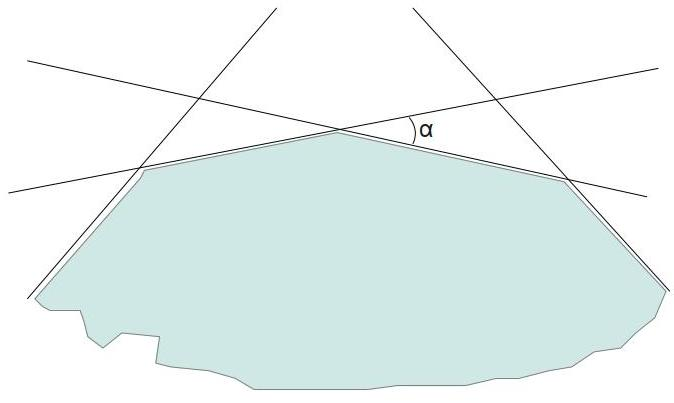
\includegraphics[clip, width=10cm]{img/contour-1.jpg}
    \caption{Смоделированный многогранник}\label{poly-model}
  \end{figure}
  \begin{figure}[h]
    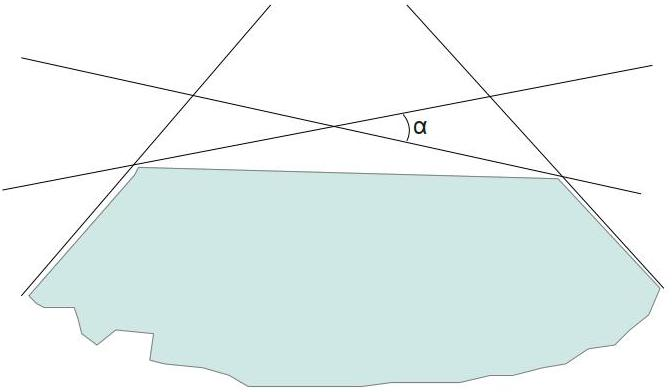
\includegraphics[clip, width=10cm]{img/contour-2.jpg}
    \caption{Реальный камень}\label{poly-real} 
  \end{figure}
\end{flushleft}
\begin{flushleft}
  В таких ситуациях происходит заведомо неоправданное усложнение структуры многогранника. В 3D-моделях
камней происходит разделение крупных граней на 2, 3, 4 более мелких. Это происходит за счет добавления 
в модель несуществующих в камне ребер. Как это может повлиять на дальнейшую работу с моделью? Если идет работа 
с одним камнем, то разница несущественна, но при массовом анализе увеличение числа ребер в 2, 3 раза приводит
к катастрофическому увеличению времени работы алгоритмов. Кроме того, лишние ребра препятствуют анализу характеристик
камня по его модели. Так, если нужно будет найти площадь самой большой грани, то когда в модели эта грань будет 
разделена на 2, то характеристика будет вычислена неверно.
\end{flushleft}
\begin{flushleft}
  Эти соображения и послужили поводом написания данной работы. В ней рассмотрены различные способы коррекции
многогранников при помощи локальных деформаций, без повторного анализа теневых контуров, то есть по уже 
построенной 3D-модели камня.
\end{flushleft}

\subsection{Что понимается под многогранником}
\begin{flushleft}
 Прежде всего следует сказать о том, каким образом задаются многогранники. Во-первых, зададается 
количество вершин и количество граней. Во-вторых, перечисляются координаты всех вершин (это тройки
чисел $x$, $y$, $z$). В-третьих, перечисляются грани. При этом указывается, сколько вершин находится в
грани, в какой плоскости она лежит (четырьмя числами $a$, $b$, $c$, $d$ из уравнения плоскости 
$a x + b y + c z + d = 0$), и список вершин, которые ее составляют.
\end{flushleft}
%\begin{flushleft}
%  Например, куб с центром в начале координат $(0, 0, 0)$ со сторонами длины 2, параллельными осям
%  координат (см. рис. ~\ref{poly-cube}), задается в данной системе следующим образом:
%\end{flushleft}
%\begin{flushleft}
%  \begin{tabular}{|c|c|}
%  \hline
%    Число вершин & Число граней \\
%  \hline
%    8 & 6 \\
%  \hline 
%  \end{tabular}
%\end{flushleft}
%\begin{flushleft}
%  \begin{tabular}{|c|c|c|c|}
%    \hline
%    Номер вершины & $x$ & $y$ & $z$ \\
%    \hline
%    0 & -1 & -1 & -1 \\
%    1 &  1 & -1 & -1 \\
%    2 &  1 &  1 & -1 \\
%    3 & -1 &  1 & -1 \\
%    4 & -1 & -1 &  1 \\
%    5 &  1 & -1 &  1 \\
%    6 &  1 &  1 &  1 \\
%    7 & -1 &  1 &  1 \\
%    \hline
%  \end{tabular}
%\end{flushleft}
%\begin{flushleft}
%  \begin{tabular}{|c|c|c|c|c|c|c|}
%    \hline
%      Номер грани & Число вершин в грани & $a$ & $b$ & $c$ & $d$ & Список вершин \\
%    \hline
%      0 & 4 &       0 & 0 &-1 &-1&      1, 0, 3, 2 \\
%      1 & 4 &       0 &-1 & 0 &-1&      0, 1, 5, 4 \\
%      2 & 4 &       1 & 0 & 0 &-1&      1, 2, 6, 5 \\
%      3 & 4 &       0 & 1 & 0 &-1&      2, 3, 7, 6 \\
%      4 & 4 &      -1 & 0 & 0 &-1&      3, 0, 4, 7 \\
%      5 & 4 &       0 & 0 & 1 &-1&      4, 5, 6, 7 \\
%    \hline
%  \end{tabular}
%\end{flushleft}
%\begin{flushleft}
%  \begin{figure}[h]
%    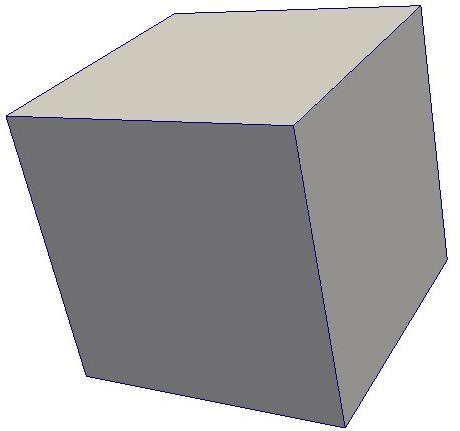
\includegraphics[clip, width=6cm]{img/cube.jpeg}
%    \caption{Куб}\label{poly-cube}
%  \end{figure}
%\end{flushleft}
\begin{flushleft}
 Таким образом задаются многогранники. В рассмотренных примерах моделей реальных камней количество
вершин варьировалось от 80 до 8000. Таким образом, во всех рассматриваемых алгоритмах встает вопрос о 
трудоемкости, то есть о времени работы.
\end{flushleft}

\section{Сглаживание смежных граней}
\subsection{Постановка задачи}
\begin{flushleft}
  Собственно, проблема была сформулирована еще во введении. Имеются две или более граней, которые находятся
в многограннике рядом с друг другом, и при этом плоскости, в которых они лежат почти совпадают, то есть угол
между их нормалями очень мал. Под словами "грани находятся друг рядом с другом" следует понимать, что на 
поверхности многогранника они занимают некоторую односвязную область. При этом нужно, чтобы существовал 
односвязный контур, который бы "охватывал" все рассматриваемые грани.
\end{flushleft}
\begin{flushleft}
 \textbf{Требуется:} вместо данной группы грани построить одну грань, которая бы состояла из точек такого 
охватывающего контура. Этой гранью нужно заменить исходную группу граней.
\end{flushleft}
\begin{flushleft}
  Иными словами, требуется удалить лишние ребра из многогранника, которые усложняют его структуру, 
разделяя одну большую грань на несколько мелких.
\end{flushleft}
\begin{flushleft}
 Можно подумать, что достаточно всего лишь построить такой охватывающий контур и на этом остановиться. Но грань, 
которая при этом получится, не будет гранью: не будет гарантии, что все ее точки будут лежать в одной плоскости.
Что мы понимаем под тем, что "точка лежит в плоскости некоторой грани"? Из математических соображений ясно, что
если $(x_{i}, y_{i}, z_{i})$ -- координаты $i$-й вершины, а $a_{k} x + b_{k} y + c_{k} z + d_{k} = 0$ -- 
уравнение плоскости $k$-й грани, то утверждение "$i$-я точка лежит в $k$-й грани" можно выразить равенством
$$
  a_{k} x_{i} + b_{k} y_{i} + c_{k} z_{i} + d_{k} = 0
$$
\end{flushleft}
\begin{flushleft}
 В нашей же теории подразумевается, что данное равенство выполнено с некоторой точностью $\varepsilon$, 
то есть
$$
  |a_{k} x_{i} + b_{k} y_{i} + c_{k} z_{i} + d_{k}| < \varepsilon
$$
При этом как правило $\varepsilon = 10^{-10}$.
\end{flushleft}
\begin{flushleft}
 Следовательно, нужно переформулировать задачу. \textbf{Требуется: } перестроить исходный многогранник таким
образом, чтобы исходная группа граней объединилась в одну грань. При этом возможно, что многогранник будет
немного изменен по своей структуре: некоторые вершины подвинуты, некоторые новые ребра могут быть добавлены.
Желательно, чтобы изменение в структуре было минимальным.
\end{flushleft}

\subsection{Описание алгоритма}
\begin{flushleft}
 Был реализован следующий алгоритм:
\end{flushleft}
\begin{flushleft}
 \textbf{1. Построение контура.} По данной группе граней строится охватывающий контур, состоящий из точек 
исходных граней.
\end{flushleft}
\begin{flushleft}
 \textbf{2. Построение средней плоскости.} По точкам полученного контура строится методом наименьших
квадратов плоскость, которая лучше всего (в смысле равенства $a_{k} x + b_{k} y + c_{k} z + d_{k} = 0$)
обеспечивает попадание исходных точек в плоскость.
\end{flushleft}
\begin{flushleft}
 Что можно сказать про построенную плоскость? Часть точек будет лежать выше нее, часть ниже, а часть довольно
хорошо (с точностью $10^{-16}$) попадет на нее. Если бы не было точек, которые лежали ниже плоскости, то 
мы бы просто рассекли многогранник полученной плоскостью и получили решение задачи. Но те точки, которые лежат 
ниже плоскости, не позволяют нам этого сделать.
\end{flushleft}
\begin{flushleft}
 \textbf{3. Поднятие точек, лежащих ниже плоскости.} Путем перестройки структуры многогранника мы добиваемся, 
чтобы \textbf{все} точки контура оказались выше построенной плоскости. Как это делается, описано в 
соответствующем пункте.
\end{flushleft}
\begin{flushleft}
 \textbf{4. Рассечение многогранника плоскостью.} После этого ничто не мешает нам просто рассечь многогранник
построенной плоскостью наименьших квадратов.
\end{flushleft}

\subsection{Примеры} 
\begin{flushleft}
  \begin{figure}[h]
    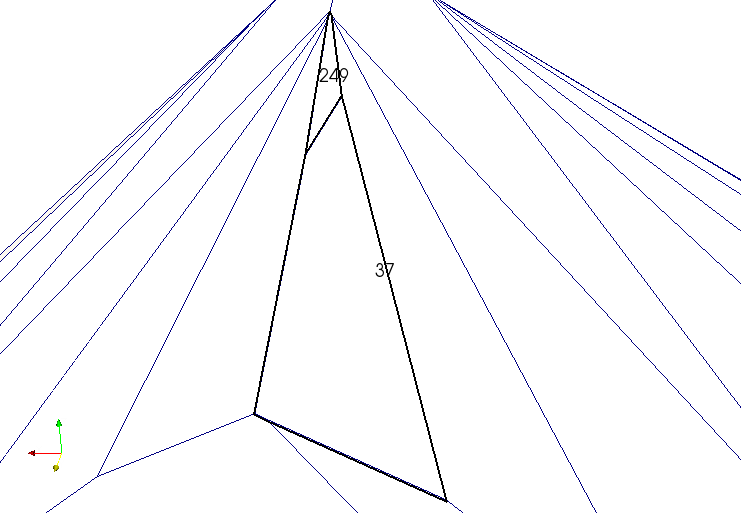
\includegraphics[clip, width=10cm]{polyhedron-2010-11-25/example-37-249.png}
    \caption{Пример двух гладко стыкующихся граней}\label{poly-join-1}
  \end{figure}
\end{flushleft}
\begin{flushleft}
  \begin{figure}[h]
    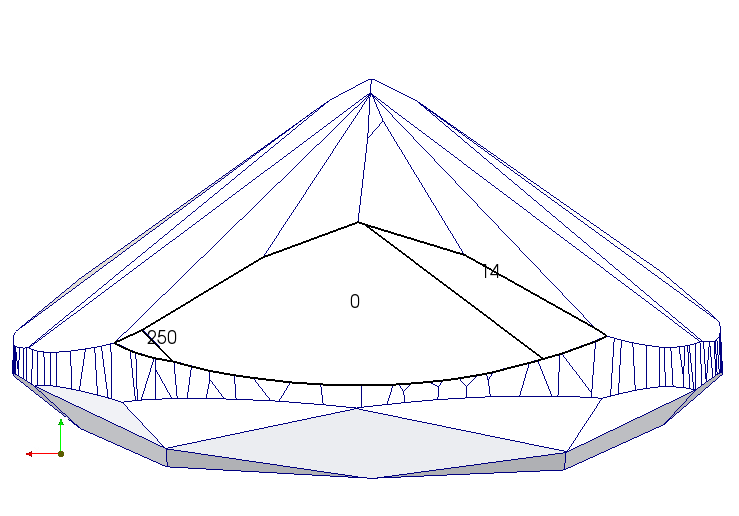
\includegraphics[clip, width=10cm]{polyhedron-2010-11-25/example-0-14-250.png}
    \caption{Пример трех гладко стыкующихся граней}\label{poly-join-2}
  \end{figure}
\end{flushleft}
\begin{flushleft}
  \begin{figure}[h]
    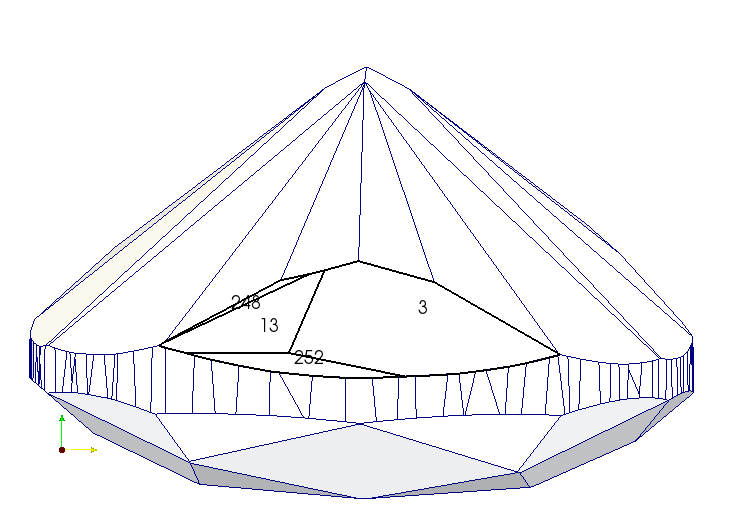
\includegraphics[clip, width=10cm]{polyhedron-2010-11-25/example-3-13-248-252.png}
    \caption{Пример четырех гладко стыкующихся граней}\label{poly-join-4}
  \end{figure}
\end{flushleft}

\subsection{Построение контура}
\begin{flushleft}
 Пусть требуется построить контур по граням с номерами $f_{0}, f_{1}, \ldots f_{n - 1}$. 
Для построения контура используется следующий алгоритм:
\end{flushleft}
\begin{flushleft}
 \textbf{1.} Заполняем массив NF следующим образом: $NF[i] = $количеству вхождений $i$-й вершины в какие-либо
грани группы $f_{0}, f_{1}, \ldots f_{n - 1}$. Для тех вершин, которые вообще не связаны с гранями данной группы, 
$NF[i] = 0$. Нам же интересны в основном те вершины, для которых $NF[i] = 1$.
\end{flushleft}
\begin{flushleft}
 \textbf{2.} Пусть $v_{0}$ - такая вершина в грани $f_{0}$, для которой $NF[v_{0}] = 1$.
\end{flushleft}
\begin{flushleft}
 \textbf{3.} $i = 0, v = v_{0}, nv = 0$
\end{flushleft}
\begin{flushleft}
 \textbf{4.} Производить следующий цикл:
\end{flushleft}
\begin{flushleft}
 \textbf{4. 1.} Производить следующий цикл пока $NF[v] = 1$:
\end{flushleft}
\begin{flushleft}
 \textbf{4. 1. 1.} Добавить вершину $v$ в контур.
\end{flushleft}
\begin{flushleft}
 \textbf{4. 1. 2.} $nv = nv + 1$
\end{flushleft}
\begin{flushleft}
 \textbf{4. 1. 3.} $v = $следующей за $v$ вершине (против часовой стрелки) в грани $f_{i}$.
\end{flushleft}
\begin{flushleft}
 \textbf{4. 2.} Добавить вершину $v$ в контур.
\end{flushleft} 
\begin{flushleft}
 \textbf{4. 3.} $nv = nv + 1$
\end{flushleft} 
\begin{flushleft}
 \textbf{4. 4.} Если $v = v_{0}$, то прервать цикл 4.
\end{flushleft} 
\begin{flushleft}
 \textbf{4. 5.} Выполнять цикл для всех $i = 0, 1, \ldots n - 1$:
\end{flushleft} 
\begin{flushleft}
 \textbf{4. 5. 1.} $v_{1} = $следующей за $v$ вершине (против часовой стрелки) в грани $f_{i}$
\end{flushleft} 
\begin{flushleft}
 \textbf{4. 5. 2.} Если $NF[v_{1}] = 1$, то прервать цикл 4.5 (т.е. этот цикл позволяет найти номер $i$ следующей
обрабатываемой нами грани).
\end{flushleft} 
\begin{flushleft}
 \textbf{4. 6.} $v = v_{1}$	
\end{flushleft} 
\begin{flushleft}
 \textbf{4. 7.} Если $v = v_{0}$, то прервать цикл 4.
\end{flushleft} 
\begin{flushleft}
 \textbf{5.} Положить $facet[0] = $грани, состоящей из построенного контура.
\end{flushleft} 
\begin{flushleft}
 \textbf{6.} Положить $facet[1] = facet[2] = \ldots = facet[n - 1] = $пустой грани.
\end{flushleft} 
\begin{flushleft}
 \textbf{7.} Осуществить ПРЕДОБРАБОТКУ многогранника.
\end{flushleft} 
\begin{flushleft}
 \textbf{8.} Удалить все висячие вершины. \textbf{Висячей} называется такая вершина, которая лежит всего в 
двух гранях. Такое происходит, когда две грани имеют два подряд идущих общих ребра.
\end{flushleft} 

\subsection{Построение средней плоскости}
\subsubsection{Метод наименьших квадратов}
\begin{flushleft}
  Для построения уравнения новой плоскости используется уже готовый алгоритм наименьших квадратов. Построенный
контур интерпретируется просто как множество точек и коэффициенты $a$, $b$, $c$ и $d$ уравнения 
$a x + b y + c z = 0$ подбираются как решение экстремальной задачи
$$
  \sum\limits_{i: A_{i} \in \pi}
	|a x_{i} + b y_{i} + c z_{i} + d |^{2} \to \min
$$
Иными словами, минимизируется сумма квадратов расстояний от точек контура до плоскости.
\end{flushleft} 

\subsubsection{TODO: Метод наименьших квадратов с весами (для учета характерных вершин)}
\begin{flushleft}
Имеется в виду, что масса грани должна быть равномерно распределена. В обычном подходе этому
мешают скопления точек, которые вынуждают плоскость пройти близко к ним, увеличивая погрешность
на изолированных точках. Для устранения этого нужно придать изолированным точкам больший вес.
делать это можно несколькими способами. \\
	\textbf{1. }Можно считать вес по длинам ребер, исходящих из точки.\\
	\textbf{2. }Можно считать вес по площади (какой?)\\
	\textbf{3. }Может быть, следует обратиться к осям инерции (?). 
\end{flushleft}


\subsection{Поднятие точек, лежащих ниже плоскости.}
%При этом возможно два подхода.\\
%	\textbf{1. }Строить грани итерационно (обходить контур).\\
%	\textbf{2. }Сначала все, что можно поднять - поднимаем, а потом - рассекаем многогранник. Этот подход 
%пытался реализовать. Подъем граней должен быть итерационным.
\begin{flushleft}
 Этот этап составляет основную содержательную часть алгоритма. Опишем его основные функции.
\end{flushleft}

\subsubsection{Основная функция}
\begin{flushleft}
 \textbf{1.} $n_{down} = $числу вершин, лежащих ниже плоскости
\end{flushleft} 
\begin{flushleft}
 \textbf{2.} Пока ($n_{down} > 1$) производить следующий цикл:
\end{flushleft} 
\begin{flushleft}
 \textbf{2. 1.} $i_{min} = $ НАЙТИ\_ПОДНИМАЕМУЮ\_ТОЧКУ
\end{flushleft} 
\begin{flushleft}
 \textbf{2. 2.} ПОДНЯТЬ\_ТОЧКУ $i_{min}$
\end{flushleft} 
\begin{flushleft}
 \textbf{2. 3.} $n_{down} = $числу вершин, лежащих ниже плоскости
\end{flushleft} 
\begin{flushleft}
 \textbf{2. 4.} Произвести ПРЕДОБРАБОТКУ многогранника
\end{flushleft} 

\subsubsection{Нахождение поднимаемой точки}
\begin{flushleft}
 \textbf{1.} $i_{min} = -1$
\end{flushleft} 
\begin{flushleft}
 \textbf{2.} Цикл (по всем точкам контура $A_{i_{0}}, A_{i_{1}}, \ldots, A_{i_{m - 1}}$,
то есть $i = i_{0}, i_{1}, \ldots, i_{m - 1}$)
\end{flushleft} 
\begin{flushleft}
 \textbf{2. 1.} Если $A_{i}$ лежит выше плоскости или на плоскости, то пропустить шаг цикла.
\end{flushleft} 
\begin{flushleft}
 \textbf{2. 2.} $d = $НАЙТИ\_ПЕРЕМЕЩЕНИЕ\_ТОЧКИ $A_{i}$
\end{flushleft} 
\begin{flushleft}
 \textbf{2. 3.} Если ($d_{min} > d$ или $i_{min} = -1$) и ($d_{min} > 10^{-15}$), то 
$d_{min} := d$, $i_{min} := i$
\end{flushleft} 

\subsubsection{Нахождение перемещения точки}
\begin{flushleft}
 Пусть находится перемещение точки $A_{i}$. Введем сначала некоторые обозначения. Пусть точка расположена
так, как показано на рис. ~\ref{pic-step-1}. Точнее говоря, пусть $f$ - главная грань, то есть грань 
построенного контура, $\pi$ - плоскость главной грани $f_{-2}, f_{-1}, f_{+1}, f_{+2}$ - соседние 
с гранью $f$ грани, $\pi_{-2}, \pi_{-1}, \pi_{+1}, \pi_{+2}$ - плоскости данных граней. При этом 
$\pi \cap \pi_{-1} \cap \pi_{+1} = A_{i}$, $\pi \cap \pi_{-2} \cap \pi_{-1} = A_{i-1}$,
$\pi \cap \pi_{+1} \cap \pi_{+2} = A_{i+1}$, где $A_{i - 1}$ - предыдущая перед точкой $A_{i}$ в контуре,
$A_{i + 1}$ - следующая перед точкой $A_{i}$ в контуре (контур организован так, что точки хранятся в нем
в направлении обхода против часовой стрелки, если смотреть извне многогранника).
\end{flushleft}
\begin{flushleft}
  \begin{figure}[h]
    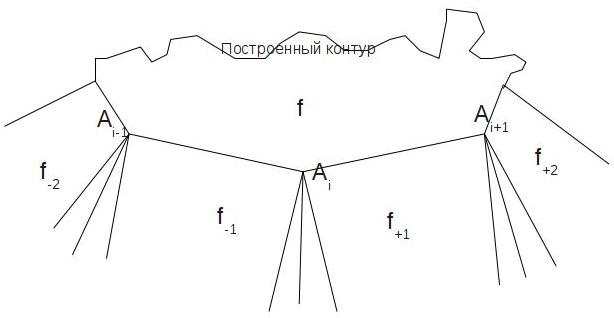
\includegraphics[clip, width=10cm]{img/pic-step-1.jpg}
    \caption{Расположение точек и граней}\label{pic-step-1}
  \end{figure}
\end{flushleft}
\begin{flushleft}
 Перед тем, как давать описание алгоритма, поясним, что значит \textbf{перемещение точки}, чтобы сделать
ясной идею данного подхода. Для простоты предположим, что степени точек $A_{i}$, $A_{i - 1}$ и $A_{i + 1}$
равны 3, то есть эти точки лежат всего в трех гранях многогранника. Это изображено на рис.
~\ref{pic-step-2}
\end{flushleft}
\begin{flushleft}
  \begin{figure}[h]
    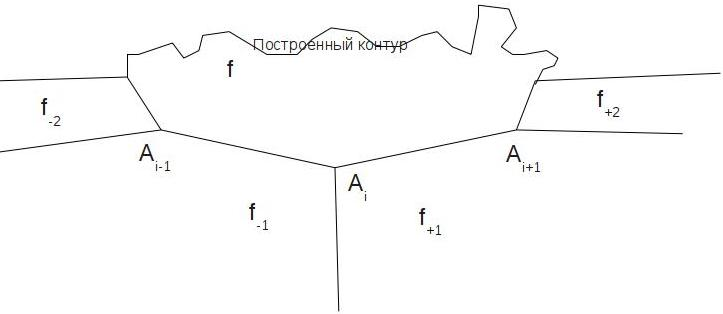
\includegraphics[clip, width=10cm]{img/pic-step-2.jpg}
    \caption{Расположение точек и граней (упрощенное)}\label{pic-step-2}
  \end{figure}
\end{flushleft}
\begin{flushleft}
  В упрощенном случае грани $f_{-1}$ и $f_{+1}$ пересекаются по ребру, одной из вершин которого является
точка $A_{i}$. Попробуем \textit{продолжить} в сторону точки $A_{i}$, то есть сдвинем точку $A_{i}$ 
по этому ребру. Такой сдвиг позволяет приближать точку, лежащую ниже плоскости, в более высокое 
положение. Производя такие сдвиги последовательно, мы надеемся поднять все точки, которые лежат ниже 
плоскости.
\end{flushleft}
\begin{flushleft}
  Насколько далеко можно произвести такой сдвиг? Ясно, что точки $A_{i - 1}$ и $A_{i + 1}$ тоже можно
сдвигать, поэтому нужно продумать алгоритм так, чтобы соответствующие ребра не пересеклись.
\end{flushleft}
\begin{flushleft}
  Поступим так: будем сдвигать точку $A_{i}$ до тех пор, пока она не попадет на продолжение одного из 
ребер, по которым двигаются точки $A_{i - 1}$ и $A_{i + 1}$. Эта идея изображена на рис.~\ref{pic-step-3}.
\end{flushleft}
\begin{flushleft}
  \begin{figure}[h]
    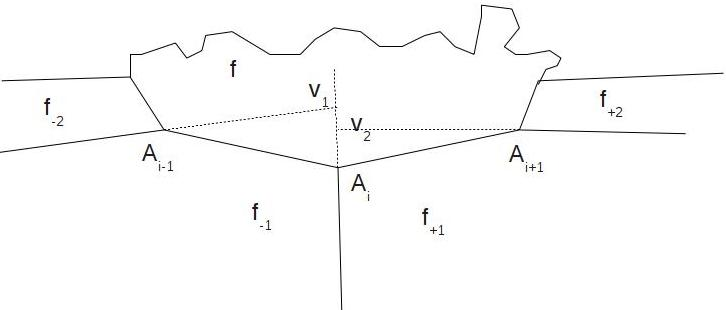
\includegraphics[clip, width=13cm]{img/pic-step-3.jpg}
    \caption{Перемещения точки $A_{i}$. TODO: $v_{-1}, v_{+1}$.}\label{pic-step-3}
  \end{figure}
\end{flushleft}
\begin{flushleft}
  В таком случае мы заменим $A_{i}$ на $v_{+1}$, а точку $A_{i + 1}$ вовсе выкинем из многогранника, а во
всех позициях, где она фигурировала, запишем точку $A_{i} = v{+1}$. Таким образом в контуре уменьшится
количество точек на 1.
\end{flushleft}
\begin{flushleft}
 Теперь мы можем описать процесс вычисления перемещения точки. Через $n$ обозначим номаль к главной грани,
то есть грани построенного контура.
\end{flushleft}
\begin{flushleft}
НАЙТИ\_ПЕРЕМЕЩЕНИЕ\_ТОЧКИ $A_{i}$\\
\verb"{"\\
\quad Если ($\pi_{-2} \parallel \pi_{+1}$)\\
\quad\verb"{"\\
\quad\quad $v_{-1} = \pi \cap \pi_{-1} \cap \pi_{+1}$\\
\quad\verb"}" \\
\quad Иначе \\
\quad\verb"{"\\
\quad\quad $v_{-1} = \pi_{-2} \cap \pi_{-1} \cap \pi_{+1}$\\
\quad\quad Если ($\pi(v_{-1}) > 0$)\\
\quad\quad \verb"{"\\
\quad\quad\quad $v_{-1} = \pi \cap \pi_{-1} \cap \pi_{+1}$\\
\quad\quad\verb"}" \\
\quad\verb"}" \\
\quad $d_{-1} = (v_{-1} - A_{i}, n)$\\

\quad Если ($\pi_{-1} \parallel \pi_{+2}$)\\
\quad \verb"{" \\
\quad\quad $v_{+1} = \pi \cap \pi_{-1} \cap \pi_{+1}$\\
\quad \verb"}"\\
\quad Иначе \\
\quad \verb"{" \\
\quad\quad $v_{+1} = \pi_{-1} \cap \pi_{+1} \cap \pi_{+2}$\\
\quad\quad Если ($\pi(v_{+1}) > 0$)\\
\quad\quad \verb"{"\\
\quad\quad\quad $v_{+1} = \pi \cap \pi_{-1} \cap \pi_{+1}$\\
\quad\quad \verb"}"\\
\quad \verb"}"\\
\quad $d_{+1} = (v_{+1} - A_{i}, n)$\\

\quad $d = min\{d_{-1}, d_{+1}\}$\\
\quad ВЕРНУТЬ $d$\\
\verb"}"\\
\end{flushleft}
\begin{flushleft}
 В общем случае кратности точек $A_{i - 1}$, $A_{i}$ и $A_{i + 1}$ могут быть больше 3. В таких случаях
точки движутся не по ребрам, а по пересечениям плоскостей, то есть не старое ребро продожается, но 
создается новое.
\end{flushleft}
\begin{flushleft}
  Зачем мы производили минимизацию по перемещению среди точек контура? Нельзя ли было просто поднимать их 
все подряд? Делается это затем, чтобы избежать самопересечений, так как если производить поднятие не
последовательно, то могут возникнуть очень большие сдвиги.
\end{flushleft}

\subsubsection{Перемещение точки}
\begin{flushleft}
 Итак, точка, которую нужно перемещать, найдена. Опишем процесс перемещения. Во-первых, повторяется 
вычисление перемещений $d_{-1}$ и $d_{+1}$. В зависимости от знака этих величин и того, какая из них 
меньше, движение определяет либо левый, либо правый сосед вершины. Алгоритм распадается на два эти случая.
\end{flushleft}
\begin{flushleft}
  Принципиальным здесь является следующее замечание. Если $\pi_{-2} \parallel \pi_{+1}$ или плоскости
$\pi_{-2}$ и $\pi_{+1}$ пересекаются, но $\pi(v_{1}) > 0$, то есть $v_{1}$ лежит выше плоскости $\pi$, 
то точки $A_{i - 1}$ и $A_{i}$ либо не сольются, либо сольются уже тогда, когда окажутся выше плоскости 
$\pi$. В этом случае не нужно объединять эти точки, но перемещать их до попадания на плоскость и оставить
топологическую структуру многограника как есть.
\end{flushleft}
\begin{flushleft}
  Далее приведем текст алгоритма:
\end{flushleft}
\begin{flushleft}
 ПОДНЯТЬ\_ВЕРШИНУ $A_{i}$\\
\verb"{"\\
\quad//Сначала найдем те же величины, что и в функции нахождения перемещения точки, дополнительно определяя
переменные $ifJoin_{-1}$ и $ifJoin_{+1}$, которые показывают, происходит ли или нет слияние вершин (см. далее).\\
\quad Если ($\pi_{-2} \parallel \pi_{+1}$)\\
\quad\verb"{"\\
\quad\quad $v_{-1} = \pi \cap \pi_{-1} \cap \pi_{+1}$\\
\quad\quad $v_{-2} = \pi \cap \pi_{-2} \cap \pi_{-1}$\\
\quad\quad $ifJoin_{-1} = FALSE$\\
\quad\verb"}" \\
\quad Иначе \\
\quad\verb"{"\\
\quad\quad $v_{-1} = \pi_{-2} \cap \pi_{-1} \cap \pi_{+1}$\\
\quad\quad $ifJoin_{-1} = TRUE$\\
\quad\quad Если ($\pi(v_{-1}) > 0$)\\
\quad\quad \verb"{"\\
\quad\quad\quad $v_{-1} = \pi \cap \pi_{-1} \cap \pi_{+1}$\\
\quad\quad\quad $v_{-2} = \pi \cap \pi_{-2} \cap \pi_{-1}$\\
\quad\quad\quad $ifJoin_{-1} = FALSE$\\
\quad\quad\verb"}" \\
\quad\verb"}" \\
\quad $d_{-1} = (v_{-1} - A_{i}, n)$\\

\quad Если ($\pi_{-1} \parallel \pi_{+2}$)\\
\quad \verb"{" \\
\quad\quad $v_{+1} = \pi \cap \pi_{-1} \cap \pi_{+1}$\\
\quad\quad $v_{+2} = \pi \cap \pi_{+1} \cap \pi_{+2}$\\
\quad\quad $ifJoin_{+1} = FALSE$\\
\quad \verb"}"\\
\quad Иначе \\
\quad \verb"{" \\
\quad\quad $v_{+1} = \pi_{-1} \cap \pi_{+1} \cap \pi_{+2}$\\
\quad\quad $ifJoin_{+1} = TRUE$\\
\quad\quad Если ($\pi(v_{+1}) > 0$)\\
\quad\quad \verb"{"\\
\quad\quad\quad $v_{+1} = \pi \cap \pi_{-1} \cap \pi_{+1}$\\
\quad\quad\quad $v_{+2} = \pi \cap \pi_{+1} \cap \pi_{+2}$\\
\quad\quad\quad $ifJoin_{+1} = FALSE$\\
\quad\quad \verb"}"\\
\quad \verb"}"\\
\quad $d_{+1} = (v_{+1} - A_{i}, n)$\\

\quadЕсли (($d_{-1} \le d_{+1}$ и $d_{-1} > 0$) или ($d_{-1} > 0$ и $d_{+1} \le 0$))\\
\quad\verb"{"\\
\quad\quad//Движение определяет левый сосед вершины\\
\quad\quadЕсли($ifJoin_{-1}$)\\
\quad\quad\verb"{"\\
\quad\quad\quad//Происходит слияние вершин\\

\quad\quad\quadЕсли (СТЕПЕНЬ($A_{i}$) > 3 и СТЕПЕНЬ($A_{i - 1}$) > 3)\\
\quad\quad\quad\verb"{"\\
\quad\quad\quad\quadСоздать новую вершину с номером $N$\\
\quad\quad\quad\quad$vertex[N] = v_{-1}$\\
\quad\quad\quad\quadДобавить точку $v_{-1}$ в грань $f_{-2}$ после точки $A_{i - 1}$\\
\quad\quad\quad\quadДобавить точку $v_{-1}$ в грань $f_{-1}$ после точки $A_{i}$\\
\quad\quad\quad\quadДобавить точку $v_{-1}$ в грань $f_{+1}$ до точки $A_{i}$\\
\quad\quad\quad\quadУдалить точку $A_{i}$ из грани $f$\\
\quad\quad\quad\quadЗаменить точку $A_{i - 1}$ в грани $f$ на точку $v_{-1}$\\
\quad\quad\quad\verb"}"\\

\quad\quad\quadИначе - Если (СТЕПЕНЬ($A_{i}$) > 3 и СТЕПЕНЬ($A_{i - 1}$) = 3)\\
\quad\quad\quad\verb"{"\\
\quad\quad\quad\quad$A_{i - 1} := v_{-1}$\\
\quad\quad\quad\quadДобавить точку $A_{i - 1}$ в грань $f_{+1}$ до точки $A_{i}$\\
\quad\quad\quad\quadУдалить точку $A_{i}$ из грани $f$\\
\quad\quad\quad\verb"}"\\

\quad\quad\quadИначе - Если (СТЕПЕНЬ($A_{i}$) = 3 и СТЕПЕНЬ($A_{i - 1}$) > 3)\\
\quad\quad\quad\verb"{"\\
\quad\quad\quad\quad$A_{i} := v_{-1}$\\
\quad\quad\quad\quadДобавить точку $A_{i}$ в грань $f_{-2}$ после точки $A_{i - 1}$\\
\quad\quad\quad\quadУдалить точку $A_{i - 1}$ из грани $f$\\
\quad\quad\quad\verb"}"\\

\quad\quad\quadИначе - Если (СТЕПЕНЬ($A_{i}$) = 3 и СТЕПЕНЬ($A_{i - 1}$) = 3)\\
\quad\quad\quad\verb"{"\\
\quad\quad\quad\quad$A_{i - 1} := v_{-1}$\\
\quad\quad\quad\quadУдалить точку $A_{i}$ из грани $f$\\
\quad\quad\quad\quadУдалить точку $A_{i}$ из грани $f_{-1}$\\
\quad\quad\quad\quadЗаменить точку $A_{i}$ в грани $f_{+1}$ на точку $A_{i - 1}$\\
\quad\quad\quad\verb"}"\\

\quad\quad\verb"}"\\
\quad\quadИначе\\
\quad\quad\verb"{"\\
\quad\quad\quad//Не происходит слияние вершин\\

\quad\quad\quadЕсли (СТЕПЕНЬ($A_{i}$) > 3 и СТЕПЕНЬ($A_{i - 1}$) > 3)\\
\quad\quad\quad\verb"{"\\
\quad\quad\quad\quadСоздать новую вершину с номером $N$\\
\quad\quad\quad\quadСоздать новую вершину с номером $N + 1$\\
\quad\quad\quad\quad$vertex[N] = v_{-2}$\\
\quad\quad\quad\quad$vertex[N + 1] = v_{-1}$\\
\quad\quad\quad\quadДобавить точку $v_{-2}$ в грань $f_{-2}$ после точки $A_{i - 1}$\\
\quad\quad\quad\quadДобавить точку $v_{-1}$ в грань $f_{-1}$ после точки $A_{i}$\\
\quad\quad\quad\quadДобавить точку $v_{-2}$ в грань $f_{-1}$ после точки $v_{-1}$\\
\quad\quad\quad\quadДобавить точку $v_{-1}$ в грань $f_{+1}$ до точки $A_{i}$\\
\quad\quad\quad\quadЗаменить точку $A_{i - 1}$ в грани $f$ на точку $v_{-2}$ \\
\quad\quad\quad\quadЗаменить точку $A_{i}$ в грани $f$ на точку $v_{-1}$\\
\quad\quad\quad\verb"}"\\

\quad\quad\quadИначе - Если (СТЕПЕНЬ($A_{i}$) > 3 и СТЕПЕНЬ($A_{i - 1}$) = 3)\\
\quad\quad\quad\verb"{"\\
\quad\quad\quad\quadСоздать новую вершину с номером $N$\\
\quad\quad\quad\quad$vertex[N] = v_{-1}$\\
\quad\quad\quad\quad$A_{i - 1} := v_{-2}$\\
\quad\quad\quad\quadДобавить точку $v_{-1}$ в грань $f_{-1}$ после точки $A_{i}$\\
\quad\quad\quad\quadДобавить точку $v_{-1}$ в грань $f_{+1}$ до точки $A_{i}$\\
\quad\quad\quad\quadЗаменить точку $A_{i}$ в грани $f$ на точку $v_{-1}$\\
\quad\quad\quad\verb"}"\\

\quad\quad\quadИначе - Если (СТЕПЕНЬ($A_{i}$) = 3 и СТЕПЕНЬ($A_{i - 1}$) > 3)\\
\quad\quad\quad\verb"{"\\
\quad\quad\quad\quadСоздать новую вершину с номером $N$\\
\quad\quad\quad\quad$vertex[N] = v_{-2}$\\
\quad\quad\quad\quad$A_{i} := v_{-1}$\\
\quad\quad\quad\quadДобавить точку $v_{-2}$ в грань $f_{-2}$ после точки $A_{i - 1}$\\
\quad\quad\quad\quadДобавить точку $v_{-2}$ в грань $f_{-1}$ после точки $A_{i}$\\
\quad\quad\quad\quadЗаменить точку $A_{i - 1}$ в грани $f$ на точку $v_{-2}$\\
\quad\quad\quad\verb"}"\\

\quad\quad\quadИначе - Если (СТЕПЕНЬ($A_{i}$) = 3 и СТЕПЕНЬ($A_{i - 1}$) = 3)\\
\quad\quad\quad\verb"{"\\
\quad\quad\quad\quad$A_{i - 1} := v_{-2}$\\
\quad\quad\quad\quad$A_{i} := v_{-1}$\\
\quad\quad\quad\verb"}"\\

\quad\quad\verb"}"\\
\quad\verb"}"\\
\quadИначе\\
\quad\verb"{"\\
\quad\quad//Движение определяет правый сосед вершины\\
\quad\quadЕсли($ifJoin_{+1}$)\\
\quad\quad\verb"{"\\
\quad\quad\quad//Происходит слияние вершин\\

\quad\quad\quadЕсли (СТЕПЕНЬ($A_{i}$) > 3 и СТЕПЕНЬ($A_{i - 1}$) > 3)\\
\quad\quad\quad\verb"{"\\
\quad\quad\quad\quadСоздать новую вершину с номером $N$\\
\quad\quad\quad\quad$vertex[N] = v_{+1}$\\
\quad\quad\quad\quadДобавить точку $v_{+1}$ в грань $f_{-1}$ после точки $A_{i}$\\
\quad\quad\quad\quadДобавить точку $v_{+1}$ в грань $f_{+1}$ до точки $A_{i}$\\
\quad\quad\quad\quadДобавить точку $v_{+1}$ в грань $f_{+2}$ до точки $A_{i + 1}$\\
\quad\quad\quad\quadУдалить точку $A_{i}$ из грани $f$\\
\quad\quad\quad\quadЗаменить точку $A_{i + 1}$ в грани $f$ на точку $A_{i + 1}$\\
\quad\quad\quad\verb"}"\\

\quad\quad\quadИначе - Если (СТЕПЕНЬ($A_{i}$) > 3 и СТЕПЕНЬ($A_{i - 1}$) = 3)\\
\quad\quad\quad\verb"{"\\
\quad\quad\quad\quad$A_{i + 1} := v_{+1}$\\
\quad\quad\quad\quadДобавить точку $A_{i + 1}$ в грань $f_{-1}$ после точки $A_{i}$\\
\quad\quad\quad\quadУдалить точку $A_{i}$ из грани $f$\\
\quad\quad\quad\verb"}"\\

\quad\quad\quadИначе - Если (СТЕПЕНЬ($A_{i}$) = 3 и СТЕПЕНЬ($A_{i - 1}$) > 3)\\
\quad\quad\quad\verb"{"\\
\quad\quad\quad\quad$A_{i} := v_{+1}$\\
\quad\quad\quad\quadДобавить точку $v_{+1}$ в грань $f_{+2}$ до точки $A_{i + 1}$\\
\quad\quad\quad\quadУдалить точку $A_{i + 1}$ из грани $f$\\
\quad\quad\quad\verb"}"\\

\quad\quad\quadИначе - Если (СТЕПЕНЬ($A_{i}$) = 3 и СТЕПЕНЬ($A_{i - 1}$) = 3)\\
\quad\quad\quad\verb"{"\\
\quad\quad\quad\quad$A_{i + 1} := v_{+1}$\\
\quad\quad\quad\quadЗаменить точку $A_{i}$ в грани $f_{-1}$ на точку $A_{i + 1}$\\
\quad\quad\quad\quadУдалить точку $A_{i}$ из грани $f_{+1}$\\
\quad\quad\quad\quadУдалить точку $A_{i}$ из грани $f$\\
\quad\quad\quad\verb"}"\\

\quad\quad\verb"}"\\
\quad\quadИначе\\
\quad\quad\verb"{"\\
\quad\quad\quad//Не происходит слияние вершин\\

\quad\quad\quadЕсли (СТЕПЕНЬ($A_{i}$) > 3 и СТЕПЕНЬ($A_{i - 1}$) > 3)\\
\quad\quad\quad\verb"{"\\
\quad\quad\quad\quadСоздать новую вершину с номером $N$\\
\quad\quad\quad\quadСоздать новую вершину с номером $N + 1$\\
\quad\quad\quad\quad$vertex[N] = v_{+1}$\\
\quad\quad\quad\quad$vertex[N + 1] = v_{+2}$\\
\quad\quad\quad\quadДобавить точку $v_{+1}$ в грань $f_{-1}$ после точки $A_{i}$\\
\quad\quad\quad\quadДобавить точку $v_{+2}$ в грань $f_{+1}$ после точки $A_{i + 1}$\\
\quad\quad\quad\quadДобавить точку $v_{+1}$ в грань $f_{+1}$ после точки $v_{+2}$\\
\quad\quad\quad\quadДобавить точку $v_{+2}$ в грань $f_{+2}$ до точки $A_{i + 1}$\\
\quad\quad\quad\quadЗаменить точку $A_{i}$ в грани $f$ на точку $v_{+1}$ \\
\quad\quad\quad\quadЗаменить точку $A_{i + 1}$ в грани $f$ на точку $v_{+2}$\\
\quad\quad\quad\verb"}"\\

\quad\quad\quadИначе - Если (СТЕПЕНЬ($A_{i}$) > 3 и СТЕПЕНЬ($A_{i - 1}$) = 3)\\
\quad\quad\quad\verb"{"\\
\quad\quad\quad\quadСоздать новую вершину с номером $N$\\
\quad\quad\quad\quad$vertex[N] = v_{+1}$\\
\quad\quad\quad\quad$A_{i + 1} := v_{+2}$\\
\quad\quad\quad\quadДобавить точку $v_{+1}$ в грань $f_{-1}$ после точки $A_{i}$\\
\quad\quad\quad\quadДобавить точку $v_{+1}$ в грань $f_{+1}$ после точки $A_{i + 1}$\\
\quad\quad\quad\quadЗаменить точку $A_{i}$ в грани $f$ на точку $v_{+1}$\\
\quad\quad\quad\verb"}"\\

\quad\quad\quadИначе - Если (СТЕПЕНЬ($A_{i}$) = 3 и СТЕПЕНЬ($A_{i - 1}$) > 3)\\
\quad\quad\quad\verb"{"\\
\quad\quad\quad\quadСоздать новую вершину с номером $N$\\
\quad\quad\quad\quad$vertex[N] = v_{+2}$\\
\quad\quad\quad\quad$A_{i} := v_{+1}$\\
\quad\quad\quad\quadДобавить точку $v_{+2}$ в грань $f_{+1}$ после точки $A_{i + 1}$\\
\quad\quad\quad\quadДобавить точку $v_{+2}$ в грань $f_{+2}$ до точки $A_{i + 1}$\\
\quad\quad\quad\quadЗаменить точку $A_{i + 1}$ в грани $f$ на точку $v_{+2}$\\
\quad\quad\quad\verb"}"\\

\quad\quad\quadИначе - Если (СТЕПЕНЬ($A_{i}$) = 3 и СТЕПЕНЬ($A_{i - 1}$) = 3)\\
\quad\quad\quad\verb"{"\\
\quad\quad\quad\quad$A_{i} := v_{+1}$\\
\quad\quad\quad\quad$A_{i + 1} := v_{+2}$\\
\quad\quad\quad\verb"}"\\

\quad\quad\verb"}"\\
\quad\verb"}"\\
\verb"}"\\

\end{flushleft}

\subsection{Утверждение о завершении алгоритма достраивания многогранника}

\begin{flushleft}
 \quadКакой смысл есть в том, что на каждом шаге данного алгоритма происходит поднятие именно той точки,
перемещение которой минимально? Нельзя ли просто по очереди поднимать вершины контура? Данное решение
было обусловлено прежде всего тем, чтобы исключить возможность образования самопересечений, которые,
как показала практика, могут образовываться при поднятии тех точек, у которых перемещение не минимально.
Далее, такой подход позволяет сформулировать и доказать три утверждения про завершение данного процесса.
\end{flushleft}

\begin{flushleft}
 \textbf{Утверждение 1.} Процесс поднятия вершин не приводит к нарушению плоскостности и образованию 
самопересечений граней и не превращает граней, являющихся выпуклыми многоугольниками, в невыпуклые.
\end{flushleft}

\begin{flushleft}
 \textit{Доказательство.} Все эти три факта можно очевидным образом проверить по тексту алгоритма:
если в грань добавляется точка, то только лежащая в этой грани, а самопересечения не могут возникнуть
и выпуклость не может нарушиться, так как точка новая точка всегда лежит еще и в соседней грани.
\end{flushleft}

\begin{flushleft}
 \textbf{Утверждение 2.} На любом шаге этого итерационного процесса найдется точка, которую можно было
бы поднять.
\end{flushleft}

\begin{flushleft}
 \textit{Доказательство.} В принципе поднять можно любую точку контура (см. алгоритм), значит найдется
 и такая, для которой расстояние минимально.
\end{flushleft}

\begin{flushleft}
 \textbf{Утверждение 3.} Процесс поднятия вершин завершается тем, что все вершины главного контура лежат
либо в плоскости, либо выше плоскости.
\end{flushleft}

\begin{flushleft}
 \textit{Доказательство.} Это утверждение доказывается тем, что на каждом шаге алгоритма происходит либо 
сдвиг одной из точек контура в положение на плоскости, либо удаление одной точки контура и сдвиг другой точки
в положение более близкое к плоскости. В силу утверждения 2 данный процесс всегда может быть продолжен,
следовательно, в результате может получиться либо пустой контур, либо контур с точками, лежащими не ниже
плоскости. Пустой контур образоваться не может, так как в силу выбора средней плоскости в контуре изначально есть
точки, лежащие выше плоскости. Они не могут быть удалены из него ни на каком шаге.
\end{flushleft}


\subsection{Рассечение модифицированного многогранника плоскостью}
\begin{flushleft}
 После того, как все точки контура оказались лежащими выше плоскости или на плоскости, можно просто 
применить алгоритм рассечения. Многогранник при этом не является обычным в смысле плоскостности граней,
поскольку в главной грани не все точки лежат в одной плоскости. Поэтому сначала рассмотрим алгоритм
рассечения обычного многогранника плоскостью, а затем скажем, что в нем нужно модифицировать, чтобы он 
работал и для нашего случая. Описанию программы рассечения посвящен следующий раздел.
\end{flushleft}

\newpage
\subsection{Тестирование алгоритма}
\begin{flushleft}
 Данный алгоритм был протестирован на 3D-моделях реальных камней. Далее перечислены 
достигнутые результаты.
\end{flushleft}

\subsubsection{Тестирование на многограннике polyhedron-2010-11-25}
\begin{flushleft}
  \begin{figure}[p]
    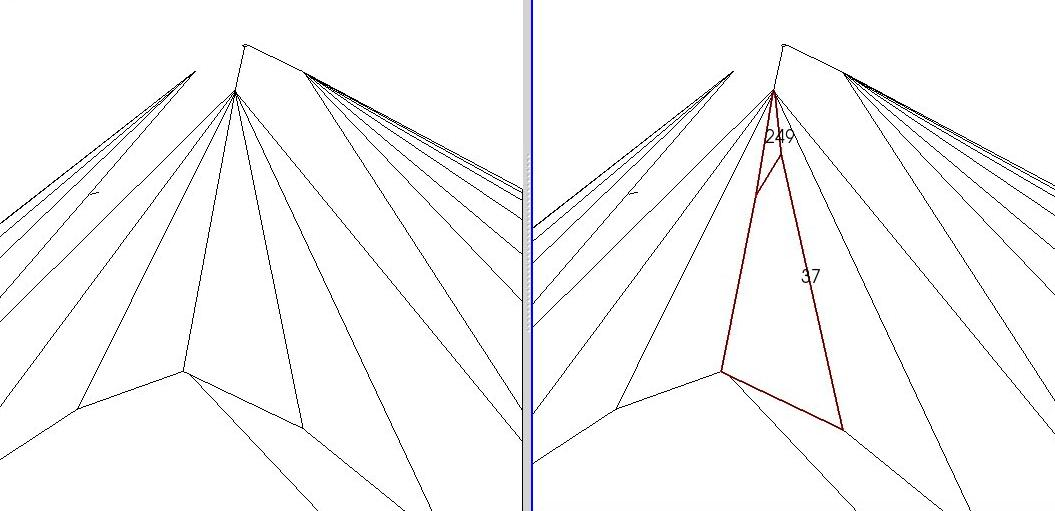
\includegraphics[width=15cm]{polyhedron-2010-11-25/join1.jpeg}
    \caption{Слияние граней 37 и 249}\label{join1}
  \end{figure}
\end{flushleft}
\begin{flushleft}
  \begin{figure}[p]
    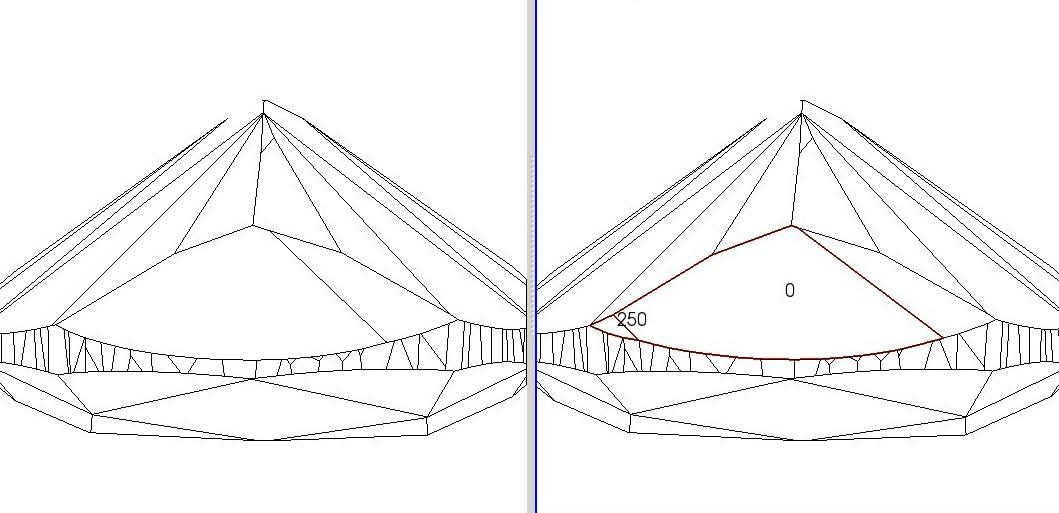
\includegraphics[width=15cm]{polyhedron-2010-11-25/join2.jpeg}
    \caption{Слияние граней 0 и 250}\label{join2}
  \end{figure}
\end{flushleft}
\begin{flushleft}
  \begin{figure}[p]
    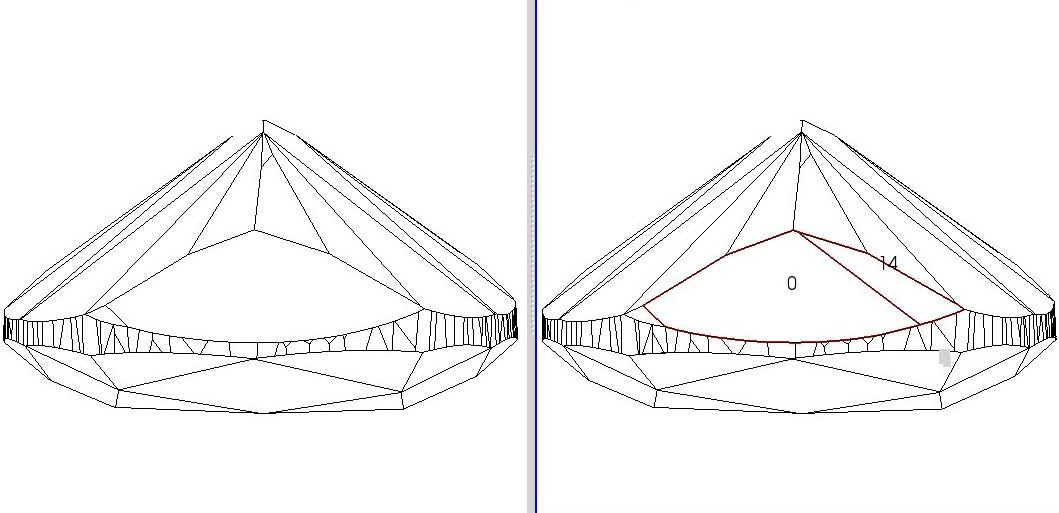
\includegraphics[width=15cm]{polyhedron-2010-11-25/join3.jpeg}
    \caption{Слияние граней 0 и 14}\label{join3}
  \end{figure}
\end{flushleft}
\begin{flushleft}
  \begin{figure}[p]
    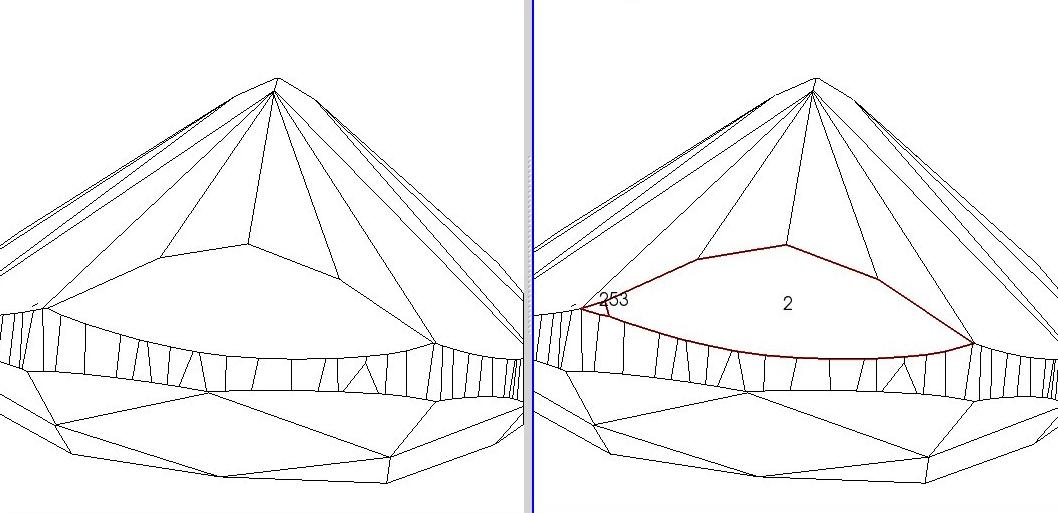
\includegraphics[width=15cm]{polyhedron-2010-11-25/join4.jpeg}
    \caption{Слияние граней 2 и 253}\label{join4}
  \end{figure}
\end{flushleft}
\begin{flushleft}
  \begin{figure}[p]
    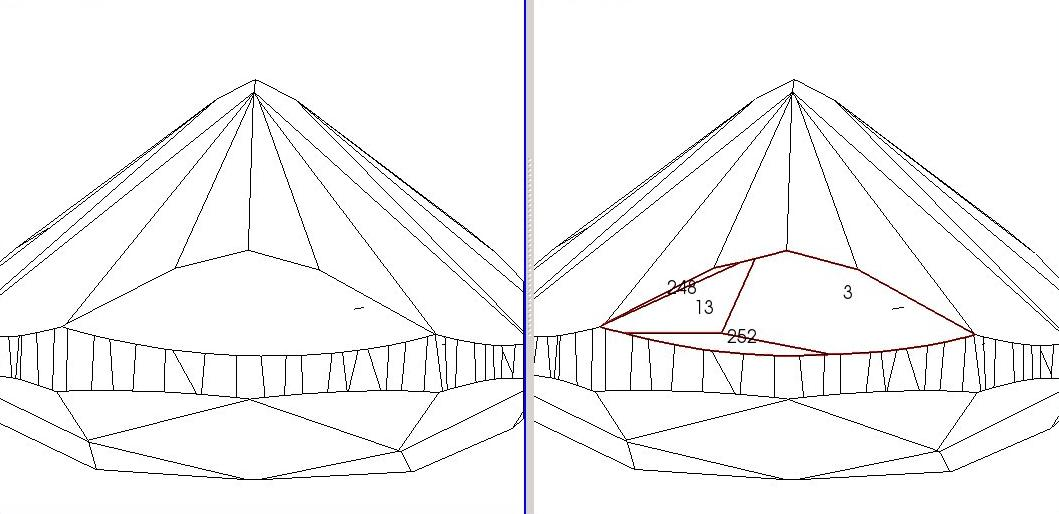
\includegraphics[width=15cm]{polyhedron-2010-11-25/join5.jpeg}
    \caption{Слияние граней 3, 13, 248 и 252}\label{join5}
  \end{figure}
\end{flushleft}
\begin{flushleft}
  \begin{figure}[p]
    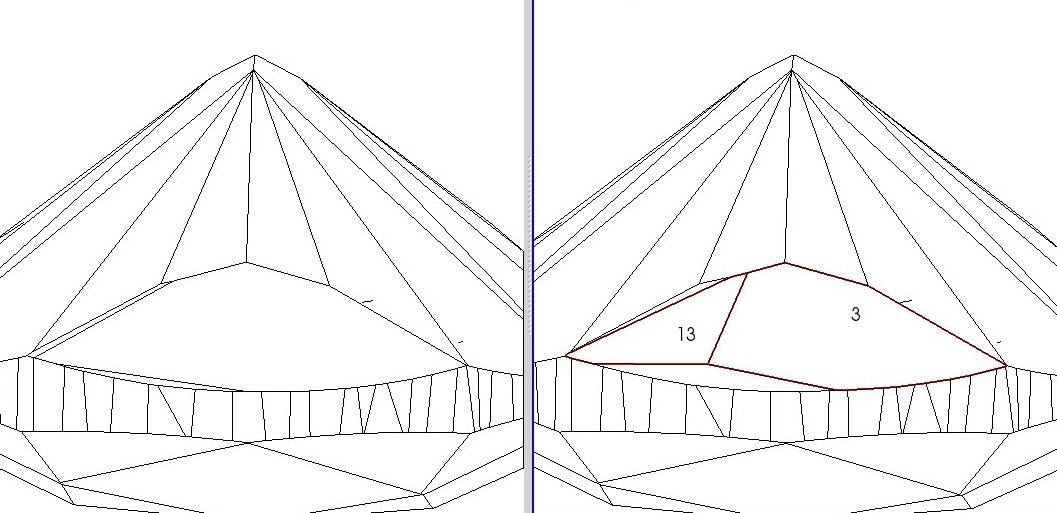
\includegraphics[width=15cm]{polyhedron-2010-11-25/join6.jpeg}
    \caption{Слияние граней 3 и 13}\label{join6}
  \end{figure}
\end{flushleft}
\begin{flushleft}
  \begin{figure}[p]
    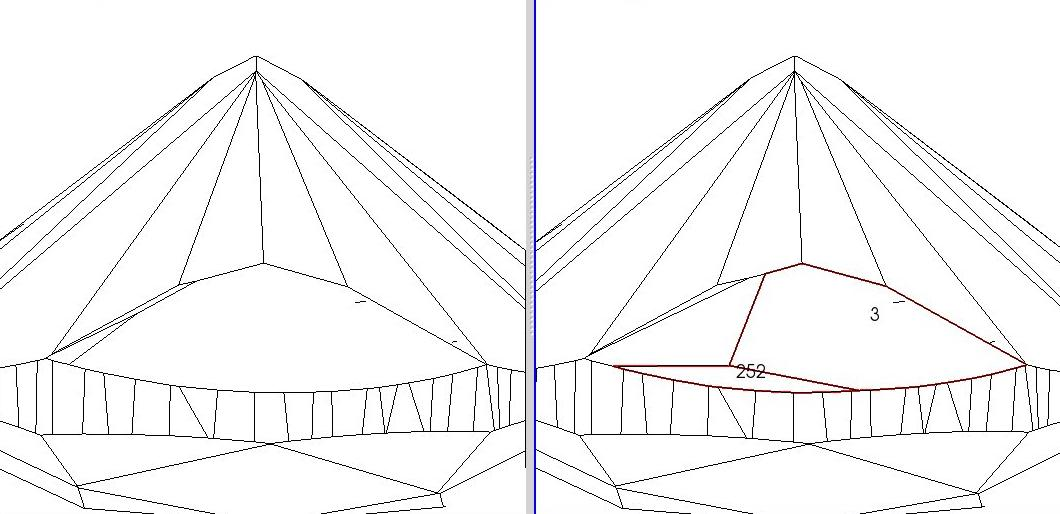
\includegraphics[width=15cm]{polyhedron-2010-11-25/join7.jpeg}
    \caption{Слияние граней 3 и 252}\label{join7}
  \end{figure}
\end{flushleft}
\begin{flushleft}
  \begin{figure}[p]
    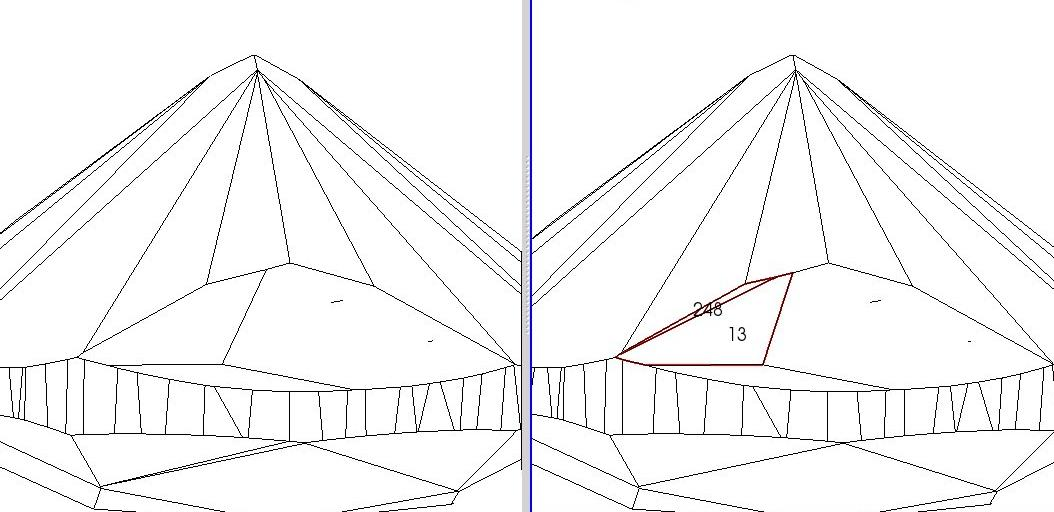
\includegraphics[width=15cm]{polyhedron-2010-11-25/join8.jpeg}
    \caption{Слияние граней 13 и 248}\label{join8}
  \end{figure}
\end{flushleft}
\begin{flushleft}
  \begin{figure}[p]
    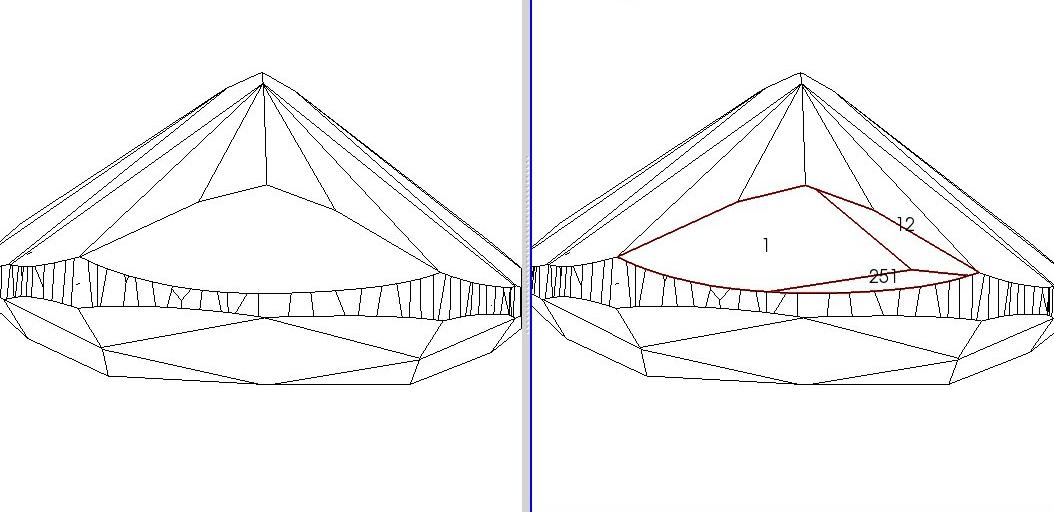
\includegraphics[width=15cm]{polyhedron-2010-11-25/join9.jpeg}
    \caption{Слияние граней 1, 12 и 251}\label{join9}
  \end{figure}
\end{flushleft}
\begin{flushleft}
  \begin{figure}[p]
    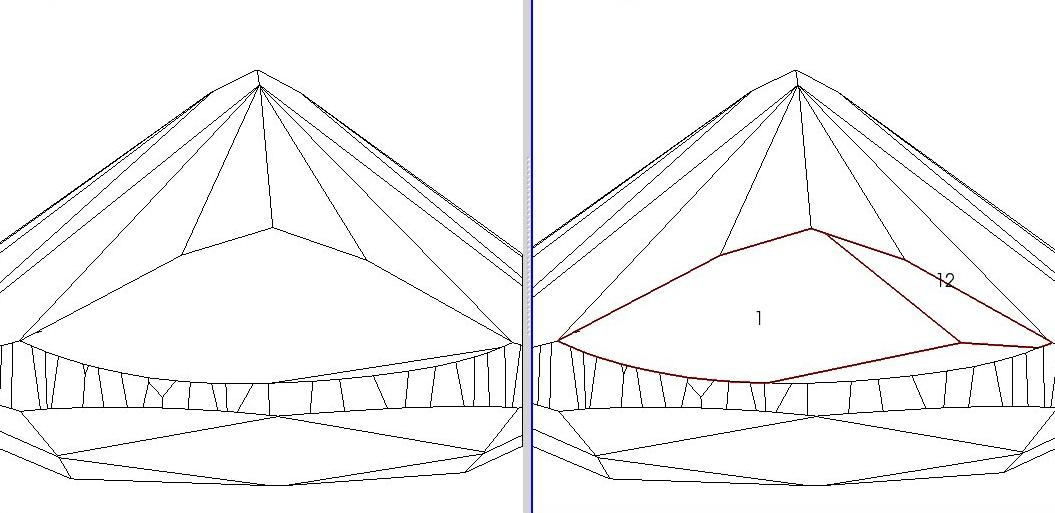
\includegraphics[width=15cm]{polyhedron-2010-11-25/join10.jpeg}
    \caption{Слияние граней 1 и 12}\label{join10}
  \end{figure}
\end{flushleft}
\begin{flushleft}
  \begin{figure}[p]
    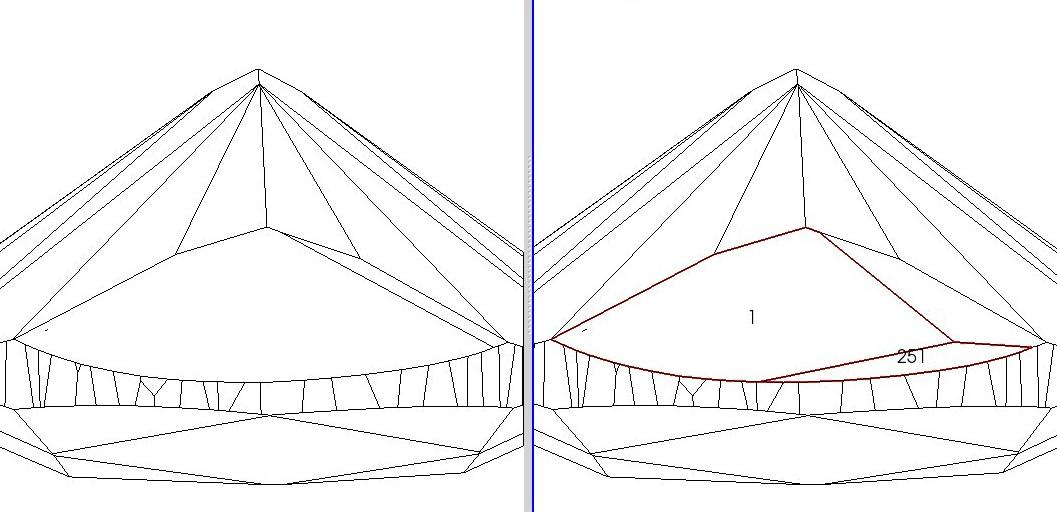
\includegraphics[width=15cm]{polyhedron-2010-11-25/join11.jpeg}
    \caption{Слияние граней 1 и 251}\label{join11}
  \end{figure}
\end{flushleft}
\begin{flushleft}
  \begin{figure}[p]
    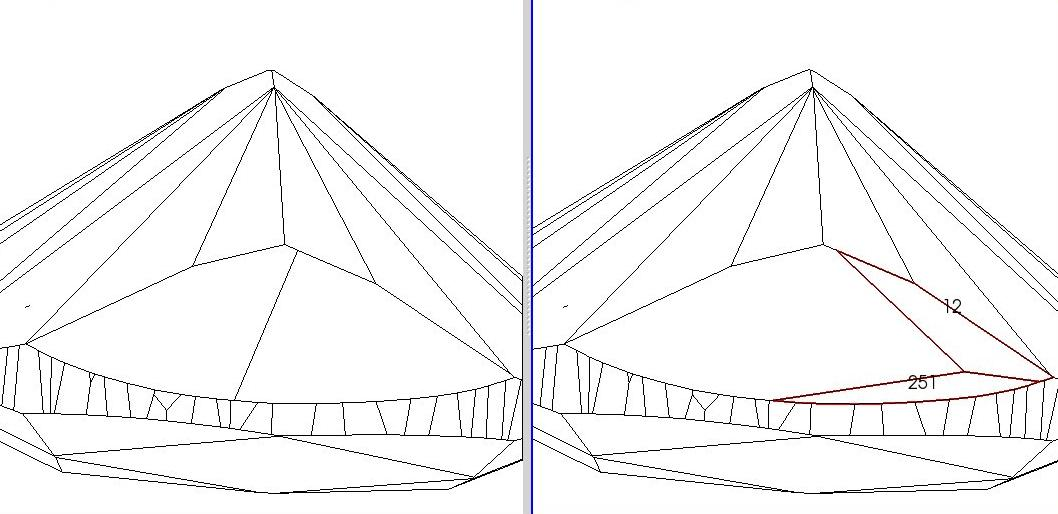
\includegraphics[width=15cm]{polyhedron-2010-11-25/join12.jpeg}
    \caption{Слияние граней 12 и 251}\label{join12}
  \end{figure}
\end{flushleft}

%\subsubsection{TODO: Тестирование на других примерах + случай трех-четырех граней}




\newpage
\section{Сечение многогранника плоскостью}

\subsection{Постановка задачи}
\begin{flushleft}
	Реализовать программу, позволяющую получать сечение произвольного многогранника
	данной плоскостью. Предусмотреть случай, когда образуется несколько компонент сечения.
\end{flushleft}

\subsection{Описание алгоритма}

\subsubsection{Этапы алгоритма}
	\begin{flushleft}
		\begin{enumerate}
			\item Предобработка многогранника
			\item Создание списков секущихся ребер для всех граней
			\item Создание компонент сечения
			\item Рассечение старых граней плоскостью
			\item Создание граней и вершин искомого многогранника
		\end{enumerate}
	\end{flushleft}

\subsubsection{Предобработка многогранника}
	\begin{flushleft}
		\begin{enumerate}
			\item В цикле для каждой грани создаются массивы номеров ее соседних граней и 
			индексов, которыми обладают ее вершины в массивах соседей
			\item В цикле для каждой вершины создается специальная структура, хранящая 
			номера граней, в которых она лежит, и индексы, которыми она в этих гранях 
			обладает
		\end{enumerate}
	\end{flushleft}
	\begin{flushleft}
		Оба цикла реализованы при помощи простого перебора
	\end{flushleft}

\subsubsection{Создание списков секущихся ребер для всех граней}
	\begin{flushleft}
		В результате выполнения этой программы образуется специальная структура, которая
		хранит в себе следующее:
	\end{flushleft}
	\begin{flushleft}
		\begin{description}
			\item[а) ]все ребра, секущиеся плоскостью, и все вершины, лежащие в плоскости,
			кроме так называемых висячих
			\item[б) ]массив упорядочивающих координат
			\item[в) ]массив номеров соседних плоскостей
			\item[г) ]массив направлений перехода
		\end{description}
	\end{flushleft}
	\begin{flushleft}
		При этом ребра хранятся упорядоченно. А именно, если рассмотреть прямую, 
		являющуюся пересечением плоскости грани $\Phi$ и секущей плоскости $\pi$, т. е.
		$l = \Phi \bigcap \pi$, то вершины и точки пересечения ребер с плоскостью 
		$\pi$ распложены на этой прямой упорядоченно (в одном из двух возможных 
		направлений).
\end{flushleft}
		\begin{flushleft}
		\begin{picture}(400,200)
		\put(100,160){\line(0,-1){160}}
		\put(100,0){\line(1,0){200}}
		\put(300,0){\line(0,1){160}}
		\put(300,160){\line(-1,0){120}}
		\put(180,160){\line(0,-1){80}}
		\put(180,80){\line(1,0){40}}
		\put(220,80){\line(0,1){40}}
		\put(220,120){\line(1,0){40}}
		\put(260,120){\line(0,-1){80}}
		\put(260,40){\line(-1,0){120}}
		\put(140,40){\line(0,1){120}}
		\put(140,160){\line(-1,0){40}}
		\multiput(5,120)(10,0){32}{\line(1,0){8}}
		\multiput(100,120)(40,0){6}{\circle*{3}}
		\put(3,120){\circle*{3}}
		\thicklines
		\put(3,120){\vector(1,0){40}}
		\thinlines
		\put(3,110){$O$}
		\put(40,125){$v$}
		\put(85,165){$A_{1}$}
		\put(85,5){$A_{2}$}
		\put(285,5){$A_{3}$}
		\put(285,165){$A_{4}$}
		\put(165,165){$A_{5}$}
		\put(165,85){$A_{6}$}
		\put(205,85){$A_{7}$}
		\put(205,125){$A_{8}$}
		\put(245,125){$A_{9}$}
		\put(240,45){$A_{10}$}
		\put(120,45){$A_{11}$}
		\put(120,165){$A_{12}$}
		\end{picture}
	\end{flushleft}

	\begin{flushleft}
		 $F(\Phi_{1}, (A_{1}, A_{2})) = (\Phi_{2}, (A_{11}, A_{12}))$
	\end{flushleft}
	\begin{flushleft}
		Если в приведенном выше примере функции подать на вход грань $\Phi_{1}$ и ребро 
		$(A_{1}, A_{2})$, то она обратится к массиву г), определит по величине $1$, соответствующей
		ребру $(A_{1}, A_{2})$, что нужно двигаться вправо, и обратится к следующему ребру массива а),
		т. е. $(A_{11}, A_{12})$ и, соответственно к плоскости $\Phi_{2}$. На выходе она возвратит 
		грань $\Phi_{2}$ и ребро $(A_{11}, A_{12})$. Направления в массиве г) будут расставлены так, 
		как показано на рисунке.
	\end{flushleft}
	\begin{flushleft}
		Как реализовано построение массива в)? Для ребра берется соседняя по этому ребру грань, которая
		определяется по структуре, построенной на этапе предобработки 1).
	\end{flushleft}
	\begin{flushleft}
		$(A_{1}, A_{2}), (A_{11}, A_{12}), (A_{5}, A_{6}), A_{8}, A_{9}, (A_{3}, A_{4})$
	\end{flushleft}
	\begin{flushleft}
		Как реализовано это упорядочение? Пусть $v$ - направляющий вектор прямой 
		$l = \Phi \bigcap \pi$, $O \in l$  - некоторая фиксированная точка на этой прямой
		$B_{i}$ - точка пересечения ребра грани с $\pi$: 
		$B_{i} = \pi \bigcap [A_{i}, A_{i + 1}]$ (или вершина грани, если сама вершина 
		лежит на $\pi$). Тогда величина
		$$
			\gamma_{i} = (v, O B_{i})
		$$
		есть координата точки $B_{i}$ на прямой $l$ в системе координат с началом в точке
		$O$ и единичным вектором $e = v$. Поэтому величины $\gamma_{i}$ могут быть 
		использованы в качестве упорядочивающих координат. 
	\end{flushleft}
	\begin{flushleft}
		Списки ребер строятся в два этапа:
		\begin{enumerate}
			\item При помощи простого перебора отыскиваются все секущиеся ребра и лежащие в 
			плоскости вершины. Список строится таким образом, чтобы он сразу был упорядоченным.
			А именно, при добавлении ребра в структуру используется двоичный поиск по 
			упорядочивающим координатам.
			\item Затем заполняются массивы из пунктов б) и в), которые будут активно 
			использоваться на дальнейших этапах алгоритма.
		\end{enumerate}
	\end{flushleft}
	\begin{flushleft}
		Какой цели служат массивы б) и в)? В основном алгоритме мы будем шагать по граням, 
		собирая секущиеся ребра и вершины компонент сечения. Чтобы определить, в какую грань 
		шагать дальше, заведена специальная функция, скажем $F$, использующая массивы б) и в).
		На вход она получает текущее ребро и грань, а на выходе возвращает следующее ребро и 
		грань.
	\end{flushleft}
	\begin{flushleft}
		В массиве г) хранятся числа $-1, 1, 0$. 
		\begin{description}
			\item[$1$ - ]если нужно двигаться вправо по списку
			\item[$-1$ - ]если нужно двигаться влево по списку
			\item[$0$ - ]если направление движения отдается на предусмотрение пользователя
		\end{description}

	\end{flushleft}
	\begin{flushleft}
		\begin{picture}(400,200)
		\put(100,160){\line(0,-1){160}}
			\put(100,160){\line(1,1){20}}
				\put(120,180){\line(1,0){40}}
		\put(100,0){\line(1,0){200}}
		\put(300,0){\line(0,1){160}}
			\put(300,0){\line(1,1){20}}
				\put(320,20){\line(0,1){160}}
		\put(300,160){\line(-1,0){120}}
			\put(300,160){\line(1,1){20}}
				\put(320,180){\line(-1,0){120}}
		\put(180,160){\line(0,-1){80}}
			\put(180,160){\line(1,1){20}}
		\put(180,80){\line(1,0){40}}
		\put(220,80){\line(0,1){40}}
			\put(220,80){\line(1,1){20}}
				\put(240,100){\line(0,1){20}}
		\put(220,120){\line(1,0){40}}
		\put(260,120){\line(0,-1){80}}
		\put(260,40){\line(-1,0){120}}
		\put(140,40){\line(0,1){120}}
			\put(140,40){\line(1,1){20}}
				\put(160,60){\line(0,1){120}}
				\put(160,60){\line(1,0){100}}
		\put(140,160){\line(-1,0){40}}
			\put(140,160){\line(1,1){20}}
		\multiput(5,120)(10,0){32}{\line(1,0){8}}
		\multiput(100,120)(40,0){6}{\circle*{3}}
		\put(90,125){$1$}
		\put(130,125){$-1$}
		\put(170,125){$1$}
		\put(210,125){$0$}
		\put(250,125){$0$}
		\put(290,125){$-1$}

		\put(3,120){\circle*{3}}
		\thicklines
		\put(3,120){\vector(1,0){40}}
		\thinlines
		\put(3,110){$O$}
		\put(40,125){$v$}
		\put(85,165){$A_{1}$}
		\put(85,5){$A_{2}$}
		\put(120,45){$A_{11}$}
		\put(120,165){$A_{12}$}
		\put(115,70){$\Phi_{1}$}
		\put(145,90){$\Phi_{2}$}

		\end{picture}
	\end{flushleft}



	\begin{flushleft}
		 $F(\Phi_{1}, (A_{1}, A_{2})) = (\Phi_{2}, (A_{11}, A_{12}))$
	\end{flushleft}
	\begin{flushleft}
		Если в приведенном выше примере функции подать на вход грань $\Phi_{1}$ и ребро 
		$(A_{1}, A_{2})$, то она обратится к массиву г), определит по величине $1$, соответствующей
		ребру $(A_{1}, A_{2})$, что нужно двигаться вправо, и обратится к следующему ребру массива а),
		т. е. $(A_{11}, A_{12})$ и, соответственно к плоскости $\Phi_{2}$. На выходе она возвратит 
		грань $\Phi_{2}$ и ребро $(A_{11}, A_{12})$. Направления в массиве г) будут расставлены так, 
		как показано на рисунке.
	\end{flushleft}
	\begin{flushleft}
		Как реализовано построение массива в)? Для ребра берется соседняя по этому ребру грань, которая
		определяется по структуре, построенной на этапе предобработки 1).
	\end{flushleft}
	\begin{flushleft}
		Для вершины также используется структура из этапа предобработки 1). А именно, перебирается
		массив содержащих эте вершину граней и проверяется, лежат ли вершины по одну или по разные 
		стороны от плоскости. Граней, в которой они лежат по разные стороны, будет всего две. Одна из 
		них - текущая, а воторую возьмем в качестве следующей. 
	\end{flushleft}
	\begin{flushleft}
	\begin{flushleft}
		\begin{picture}(260,200)
		\put(20,180){\line(0,-1){120}}
		\put(20,60){\line(1,0){60}}
		\put(20,180){\line(1,0){200}}
		\put(220,180){\line(0,-1){120}}
		\put(220,60){\line(-1,0){60}}
		\multiput(80,60)(10,0){8}{\line(1,0){8}}
		\put(120,160){\line(-3,-4){60}}
		\put(120,160){\line(3,-4){60}}
		\put(100,40){\line(1,6){20}}
		\put(140,40){\line(-1,6){20}}
		\put(60,80){\line(1,-1){40}}
		\put(100,40){\line(1,0){40}}
		\put(140,40){\line(1,1){40}}
		\multiput(60,80)(10,0){12}{\line(1,0){8}}
		
		\put(115,165){$A$}
		\put(45,85){$B_{1}$}
		\put(85,30){$B_{2}$}
		\put(145,30){$B_{3}$}
		\put(180,85){$B_{4}$}
		\put(95,105){$\Phi_{1}$}
		\put(115,95){$\Phi_{2}$}
		\put(135,105){$\Phi_{3}$}
		\put(180,130){$\Phi_{4}$}
		\put(180,130){\vector(-2,-1){20}}

		\end{picture}
	\end{flushleft}
	\end{flushleft}
	\begin{flushleft}
		В примере на приведенном выше рисунке для вершины $A$ искомыми гранями будут $\Phi_{1}$
		и $\Phi_{2}$, поскольку вершины $B_{1}$ и 
		$B_{2}$, $B_{3}$ и $B_{4}$ лежат по разные стороны от плоскости $\pi$.
	\end{flushleft}
	\begin{flushleft}
		Заметим, что для вершины предусмотрена одна исключительная ситуация: если в массиве г) на 
		соответствуюшей позиции стоит $0$, то следущая грань не ищется, а считается, что в этой точке
		следующей гранью является текушая.
	\end{flushleft}
	\begin{flushleft}
		Как реализовано построение массива г)? При реализации используется следущая идея. Грань - 
		замкнутое плоское множество. Рассмотрим прямую $l = \pi \bigcap \Phi$ и будем двигаться 
		непрерывно вдоль нее из бесконечности, положив начальное направление равным $\nu = -1$. Когда мы 
		попадаем на грань, то меняем направление: $\nu = \nu \cdot (-1) = 1$ и приписываем его задействованному
		ребру или вершине. Продолжаем двигаться дальше. Если мы оказались вне грани, то поменяем 
		направление: $\nu = \nu \cdot (-1) = -1$ и приписываем его задействованному ребру или вершине.
		В промежутке между сменами $\nu$ нам могли попадаться вершины, лежащие на плоскости. Если они
		висячие, то пропустим их, как было сказано выше. Если же не являются, то припишем им направление,
		равное $0$.
	\end{flushleft}
		\begin{flushleft}
		\begin{picture}(440,120)
		\put(80,40){\line(1,2){20}}
		\put(100,80){\line(1,0){40}}
		\put(140,80){\line(1,2){20}}
		\put(160,120){\line(1,0){40}}
		\put(200,120){\line(1,-2){20}}
		\put(220,80){\line(1,0){80}}
		\put(300,80){\line(1,-2){20}}
		\put(320,40){\line(1,2){20}}
		\put(340,80){\line(1,0){40}}
		\put(380,80){\line(1,-2){20}}
		\put(400,40){\line(-1,-2){20}}
		\put(380,0){\line(-1,0){280}}
		\put(100,0){\line(-1,2){20}}

		\put(80,40){\circle*{3}}
		\put(100,80){\circle*{3}}
		\put(140,80){\circle*{3}}
		\put(160,120){\circle*{3}}
		\put(200,120){\circle*{3}}
		\put(220,80){\circle*{3}}
		\put(260,80){\circle*{3}}
		\put(300,80){\circle*{3}}
		\put(320,40){\circle*{3}}
		\put(340,80){\circle*{3}}
		\put(380,80){\circle*{3}}
		\put(400,40){\circle*{3}}
		\put(380,0){\circle*{3}}
		\put(100,0){\circle*{3}}

		\multiput(5,80)(10,0){43}{\line(1,0){8}}
		\thicklines
		\put(0,80){\vector(1,0){40}}

		\put(105,65){$1$}
		\put(140,65){$0$}
		\put(220,65){$0$}
		\put(260,65){$0$}
		\put(285,65){$-1$}
		\put(345,65){$1$}
		\put(365,65){$-1$}

		\end{picture}
	\end{flushleft}

	\begin{flushleft}
		Если применить процесс к такой грани, то направления будут приписаны так, как показано 
		на рисунке.
	\end{flushleft}
	\begin{flushleft}
		Как реализовать этот процесс при помощи алгоритма?
	\end{flushleft}
	\begin{flushleft}
		Если точка пересечения грани с плоскотью одна, то она висячая, и рассмотрение такой грани можно 
		отбросить. Если их две, то построение тривиально: одной приписываем направление $1$, а другой - 
		$(-1)$.
	\end{flushleft}
	\begin{flushleft}
		\begin{picture}(180,80)
		\put(80,40){\line(1,2){20}}
		\put(100,80){\line(1,0){40}}
		\put(140,80){\line(0,-1){80}}
		\put(140,0){\line(-1,0){40}}
		\put(100,0){\line(-1,2){20}}

		\put(80,40){\circle*{3}}
		\put(100,80){\circle*{3}}
		\put(140,80){\circle*{3}}
		\put(140,40){\circle*{3}}
		\put(140,0){\circle*{3}}
		\put(100,0){\circle*{3}}

		\multiput(5,40)(10,0){17}{\line(1,0){8}}
		\thicklines
		\put(0,40){\vector(1,0){40}}

		\put(75,30){$1$}
		\put(145,30){$-1$}

		\end{picture}
	\end{flushleft}
	\begin{flushleft}
		В общем случае точек пересечения не менее трех, и тогда запускаетя второй цикл по массиву вершин 
		грани. При этом используются 2 вспомогательные переменные: $s$ и $\nu$. $\nu$ обозначает, 
		находится ли шаг цикла внутри ($1$) или вне ($-1$) грани. $s$ обозначает, находится ли шаг цикла
		выше ($1$) или ниже ($-1$) секущей плоскости. Для простоты алгоритм начинается с самой левой точки
		пересечения и идет по списку вершин грани в таком направлении, двигаясь по которому, мы получим
		следующую точку в списке за самой левой точкой (а не самую правую, как если бы выбрать 
		противоположное направление).
	\end{flushleft}
	\begin{flushleft}
		$v_{0}$ = первой вершине\\
		$v_{+1}$ = следующей за $v_{0}$ вершине\\
		цикл(по всем вершинам грани)\\
		\verb"{"\\
		\quad$s_{0}$ = знак($v_{0}$)\\
		\quad$s_{+1}$ = знак($v_{+1}$)\\
		\quadесли($s_{0} = 0$ или $s_{0} \cdot s_{+1} = -1$)\\
		\quad\verb"{"\\
		\quad\quadесли($s_{+1} = -s$ \quad\verb"//"следующая вершина уходит на другую сторону\\
		\quad\quad\quadили $s_{0} = 0$ и $\nu = -1$ \quad\verb"//"произошло вхождение точки на плоскость\\
		\quad\quad\quadили $s_{0} \cdot s_{+1} = -1$) \quad\verb"//"произошло пересечение по ребру\\
		\quad\quad\verb"{"\\
		\quad\quad\quad$\nu = -\nu$\\
		\quad\quad\quad$s = -s$\\
		\quad\quad\quad$n = \nu$\\
		\quad\quad\quad$f$ = найти следующую грань\\
		\quad\quad\verb"}"\\
		\quad\quadиначе\\
		\quad\quad\verb"{"\\
		\quad\quad\quad$n = 0$\\
		\quad\quad\quad$f = \Phi$\\
		\quad\quad\verb"}"\\
		\quad\verb"}"\\
		\quadесли($s_{0} \cdot s_{+1} = -1$)\\
		\quad\verb"{"\\
		\quad\quadнайти ребро $(v_{0}, v_{+1})$ в списке\\
		\quad\quadприписать ему направление $n$ и соседнюю грань $f$\\
		\quad\verb"}"\\
		\quadесли($s_{0} = 0$)\\
		\quad\verb"{"\\
		\quad\quadнайти вершину $v_{0}$ в списке\\
		\quad\quadприписать ей направление $n$ и соседнюю грань $f$\\
		\quad\verb"}"\\
		\verb"}"\\
	\end{flushleft}

	\begin{flushleft}
		На самом деле данный алгоритм описывает не совсем тот процесс, который был описан выше.
	\end{flushleft}

	\begin{flushleft}
		\begin{picture}(400,200)
		\put(100,160){\line(0,-1){160}}
		\put(100,0){\line(1,0){200}}
		\put(300,0){\line(0,1){160}}
		\put(300,160){\line(-1,0){120}}
		\put(180,160){\line(0,-1){80}}
		\put(180,80){\line(1,0){40}}
		\put(220,80){\line(0,1){40}}
		\put(220,120){\line(1,0){40}}
		\put(260,120){\line(0,-1){80}}
		\put(260,40){\line(-1,0){120}}
		\put(140,40){\line(0,1){120}}
		\put(140,160){\line(-1,0){40}}
		\multiput(5,120)(10,0){32}{\line(1,0){8}}
		\multiput(100,120)(40,0){6}{\circle*{3}}
		\put(3,120){\circle*{3}}
		\thicklines
		\put(3,120){\vector(1,0){40}}
		
		\put(90,125){\vector(0,1){30}}
		\put(110,155){\vector(1,0){30}}
		\put(145,110){\vector(0,-1){30}}
		\put(190,45){\vector(1,0){30}}
		\put(265,70){\vector(0,1){30}}
		\put(250,115){\vector(-1,0){30}}
		\put(175,130){\vector(0,1){30}}
		\put(190,155){\vector(1,0){30}}
		\put(305,90){\vector(0,-1){30}}
		\put(170,5){\vector(-1,0){30}}

		\put(85,165){$A_{1}$}
		\put(85,5){$A_{2}$}
		\put(285,5){$A_{3}$}
		\put(285,165){$A_{4}$}
		\put(165,165){$A_{5}$}
		\put(165,85){$A_{6}$}
		\put(205,85){$A_{7}$}
		\put(205,125){$A_{8}$}
		\put(245,125){$A_{9}$}
		\put(240,45){$A_{10}$}
		\put(120,45){$A_{11}$}
		\put(120,165){$A_{12}$}
		\end{picture}
	\end{flushleft}
	
	\begin{flushleft}
		А именно, он перебирает ребра не в порядке их нахождения в списке. Впрочем, очевидно, что
		параметр $s$ меняется нужным образом: количество подъемов равно количеству спусков за счет
		того, что не рассматриваются висячие вершины. А параметр $\nu$ меняется четное число раз, и
		как раз в тех точках, где меняется параметр $s$. Значит, в результате алгоритма ребрам будут
		приписаны искомые направления.
	\end{flushleft}

	\begin{flushleft}
		Построение массивов в) и г) выделено в отдельный цикл, т. к. в алгоритме существенно, чтобы
		обход начинался с самой левой вершины в списке, а это возможно организовать только после 
		того, как все секущиеся ребра и вершины зарегистрированы.
	\end{flushleft}


\subsubsection{Создание компонент сечения}	
	\begin{flushleft}
		Организуется простой перебор полученных списков. Выбирается начальное ребро и при помощи 
		функции перехода $F$ ищутся те ребра, которые за ним следуют, до тех пор, пока цикл не придет
		к исходному ребру. Если в результате количество задействованных ребер меньше, чем то, которое
		хранится в списках, то выбирается какое-нибудь еще не задействованное ребро и цикл 
		повторяется. В результате будет проделано ровно столько циклов, сколько компонент в сечении
		многогранника. Секущиеся ребра и вершины, образующие вершины этих компонент, запоминаются в 
		специальных структурах.
	\end{flushleft}

\subsubsection{Рассечение старых граней плоскостью}	
	\begin{flushleft}
		Используются построенные в пункте 2 списки.
	\end{flushleft}

	\begin{flushleft}
		пока(в списке есть неиспользованные ребра \verb"/" вершины)\\
		\verb"{"\\
		\quad$(v_{0}^{0}, v_{1}^{0})$ = неиспользованное ребро или вершина\\
		\quad$(v_{0}, v_{1}) = (v_{0}^{0}, v_{1}^{0})$\\
		\quadделать\quad\verb"//"цикл А\\
		\quad\verb"{"\\
		\quad\quadдобавить ребро $(v_{0}, v_{1})$\\
		\quad\quad$(v_{0}, v_{1})$ = следующее за $(v_{0}, v_{1})$ ребро\\
		\quad\quad$s_{+1}$ = знак следующей за $v_{0}$\\
		\quad\quad$s_{-1}$ = знак предыдущей для $v_{0}$\\
		\quad\verb"}"пока($s_{-1} = 0$ и $s_{+1} = 0$)\\
		\quadдобавить ребро $(v_{0}, v_{1})$\\
		\quadвыбрать положительное направление\\
		\quad$I$ = следующая вершина в положительном направлении\\
		\quadделать\quad\verb"//"цикл Б\\
		\quad\verb"{"\\
		\quad\quadдобавить вершину $I$\\
		\quad\quad$I$ = следующая за $I$ в положительном направлении\\
		\quad\quad$s_{0}$ = знак($I$)\\
		\quad\verb"}"пока($s_{0} = 1$)\\
		\quadесли($s_{0} = 0$)\\
		\quad\verb"{"\\
		\quad\quad$v_{0} = v_{1} = I$\\
		\quad\verb"}"\\
		\quadесли($s_{0} = -1$)\\
		\quad\verb"{"\\
		\quad\quad$v_{0} = I$\\
		\quad\quad$v_{1}$ = предыдущей вершине для $I$\\
		\quad\verb"}"\\		
		\verb"}"пока($v_{0} \ne v_{0}^{0}$ или $v_{1} \ne v_{1}^{0}$)\\		
	\end{flushleft}
	
	\begin{flushleft}
		Если оказалось, что в самом начале список пуст, то нужно попробовать найти в грани
		положительные вершины. Если таковых нет, то грань удаляется. Если такие есть, то все
		вершины являюся либо положительными, либо висячими, и грань целиком лежит выше плоскости,
		и тогда ее нужно оставить без изменения.
	\end{flushleft}
	
	\begin{flushleft}
		\begin{picture}(400,200)
		\put(100,160){\line(0,-1){160}}
		\put(100,0){\line(1,0){200}}
		\put(300,0){\line(0,1){160}}
		\put(300,160){\line(-1,0){120}}
		\put(180,160){\line(0,-1){80}}
		\put(180,80){\line(1,0){40}}
		\put(220,80){\line(0,1){40}}
		\put(220,120){\line(1,0){40}}
		\put(260,120){\line(0,-1){80}}
		\put(260,40){\line(-1,0){120}}
		\put(140,40){\line(0,1){120}}
		\put(140,160){\line(-1,0){40}}
		\multiput(5,120)(10,0){32}{\line(1,0){8}}
		\put(3,130){$+$}
		\put(3,110){$-$}

		\thicklines

		\put(100,160){\vector(1,0){20}}
		\put(120,160){\vector(1,0){20}}
		\put(140,160){\vector(0,-1){20}}
		\put(140,140){\vector(0,-1){20}}
		\put(140,120){\vector(-1,0){20}}
		\put(120,120){\vector(-1,0){20}}
		\put(100,120){\vector(0,1){20}}
		\put(100,140){\vector(0,1){20}}

		\multiput(180,120)(20,0){6}{\vector(1,0){20}}
		\put(300,120){\vector(0,1){20}}
		\put(300,140){\vector(0,1){20}}
		\multiput(300,160)(-20,0){6}{\vector(-1,0){20}}
		\put(180,160){\vector(0,-1){20}}
		\put(180,140){\vector(0,-1){20}}

		\put(120,105){А}
		\put(200,105){А}
		\put(280,105){А}
		\put(120,165){Б}
		\put(240,165){Б}

		\end{picture}
	\end{flushleft}

	\begin{flushleft}
		Алгоритм найдет 2 компоненты для такой грани. Стрелки на рисунке показывают порядок, в 
		котором будут находиться вершины. А соответствует циклу А, а Б - циклу Б из алгоритма выше.
	\end{flushleft}
	
	\begin{flushleft}
		В цикле А движение происходит по плоскости, пока мы находимся внутри грани. Как только мы
		выходим за ее пределы, шагаем вверх и двигаемся до тех пор, пока снова не опустимся на 
		плоскость (это соответствует циклу Б).
	\end{flushleft}

\subsubsection{Создание граней и вершин искомого многогранника}	
	\begin{flushleft}
		\begin{enumerate}
			\item По мере создания списков секущихся ребер и вершин возникающие ребра запоминаются, 
			т. к. они в пересечении с плоскостью создают новые вершины. Для запоминания используется 
			структура типа множество. 
			\item Когда выполнены этапы 2 - 4, начинается создание новых граней по секущимся ребрам,
			которые были сохранены во время этапов 3 и 4. При создании вершинам присваиваются номера
			$N + i$, где $N$ - количество вершин в старом многограннике, $i$ - номер вершины в 
			структуре типа множество.
			\item После этого удаляются все отрицательные вершины и те грани, в которых нет 
			положительных вершин.
			\item Затем вершины и грани перенумеровываются, чтобы в массивах не было пустых элементов.
		\end{enumerate}
	\end{flushleft}

\subsection{Тестирование алгоритма}
	\begin{flushleft}
		Алгоритм был протестирован на модельных и реальных примерах, в том числе таких, в которых
		возникают многокомпонентные сечения и грани, которые пи рассечении распадаются на несколько
		компонент-граней.
	\end{flushleft}
	\begin{flushleft}
		Во всех приведенных ниже иллюстрациях слева изображен исходный многогранник, справа - его 
		сечение. Компоненты сечения раскрашены ярко-красным цветом, а те грани, которые образовались
		в результате рассечения старых граней плоскостью, раскрашены темно-красным цветом.
	\end{flushleft}

\newpage
\subsubsection{Тестирование на модельном многограннике cube-cutted}
	\begin{flushleft}
%		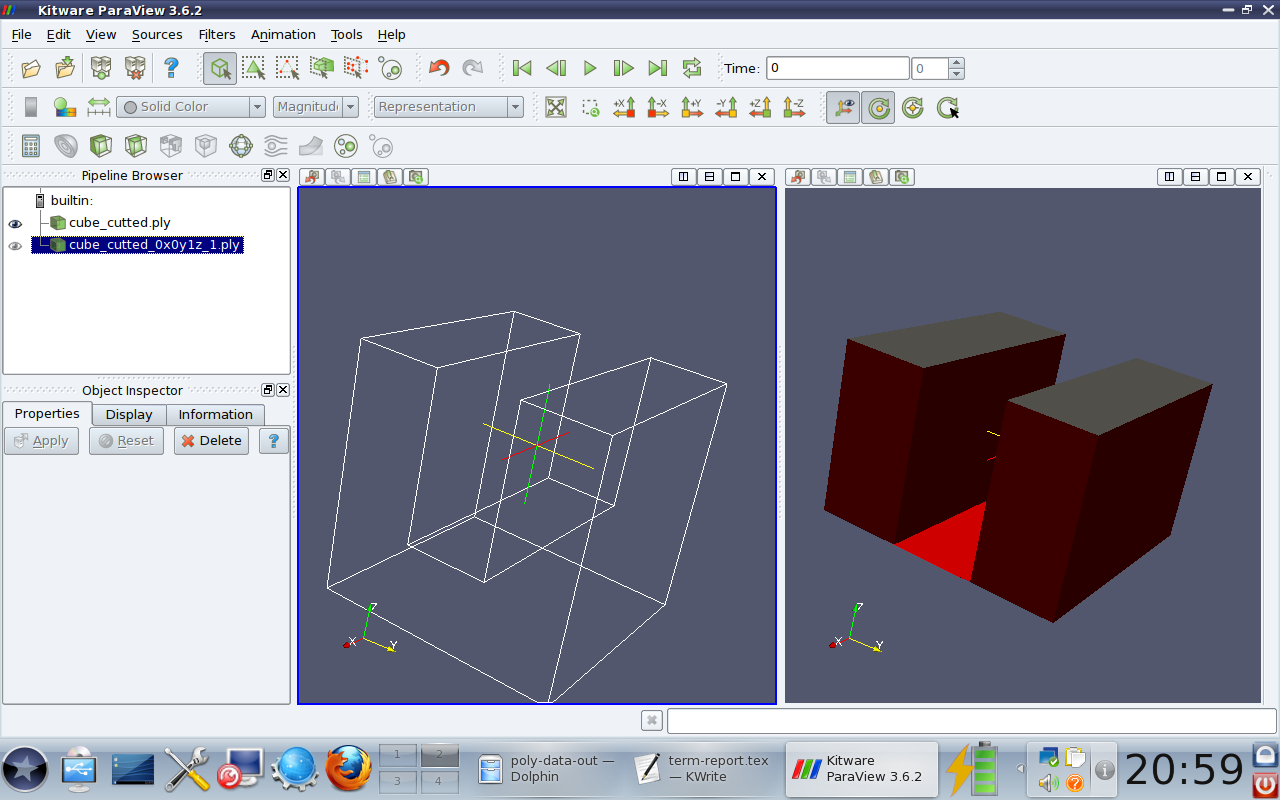
\includegraphics[trim = 220 65 10 140, clip, width=15cm]{cube-cutted/1.png}
		\begin{figure}[h]
		    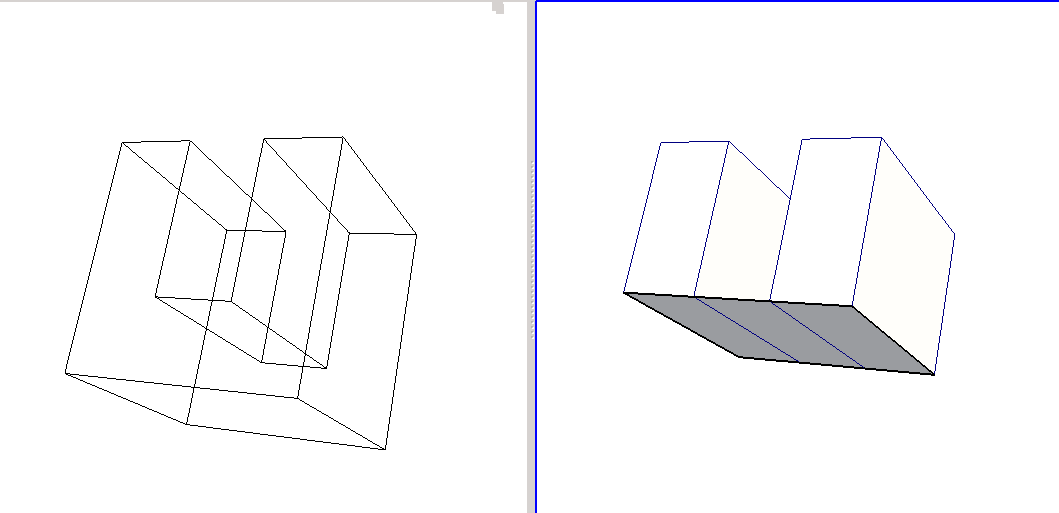
\includegraphics[width=15cm]{cube-cutted/cube-cutted-1.png}
		    \caption{Сечение многогранника cube-cutted плоскостью $z = 1$. В данном случае образуется 1
		компонента сечения. Заметим, что она состоит из всего одной грани, несмотря на то, что
		существует грань исходного многогранника, которая целиком содержится в компоненте.}
		    \label{cube-cutted-1}
		\end{figure}
		
	\end{flushleft}
	\begin{flushleft}
		\begin{figure}[h]
		    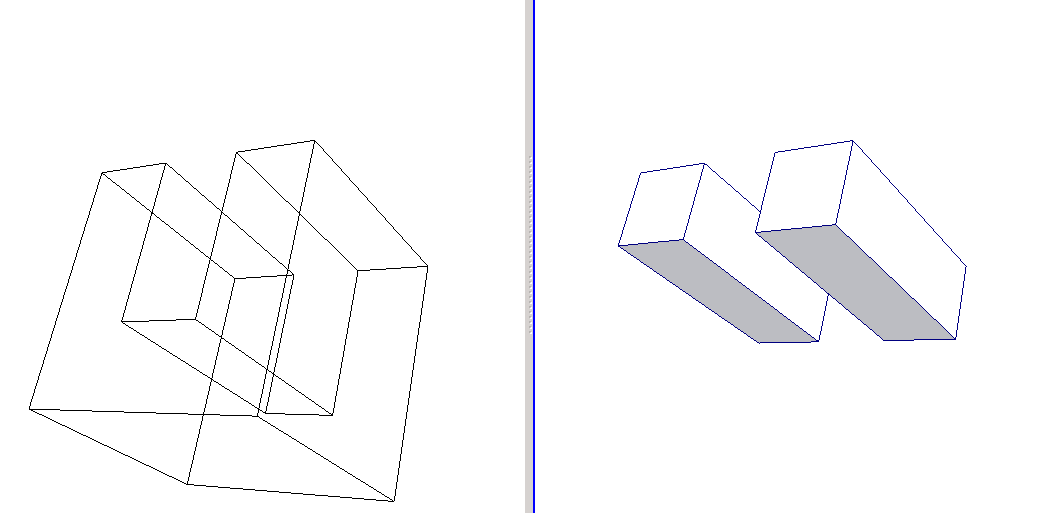
\includegraphics[width=15cm]{cube-cutted/cube-cutted-2.png}
		    \caption{Сечение многогранника cube-cutted плоскостью $z = 2$. В данном случае образуется 2
		компоненты сечения.}
		    \label{cube-cutted-2}
		\end{figure}
	\end{flushleft}
	\begin{flushleft}
		\begin{figure}[h]
		    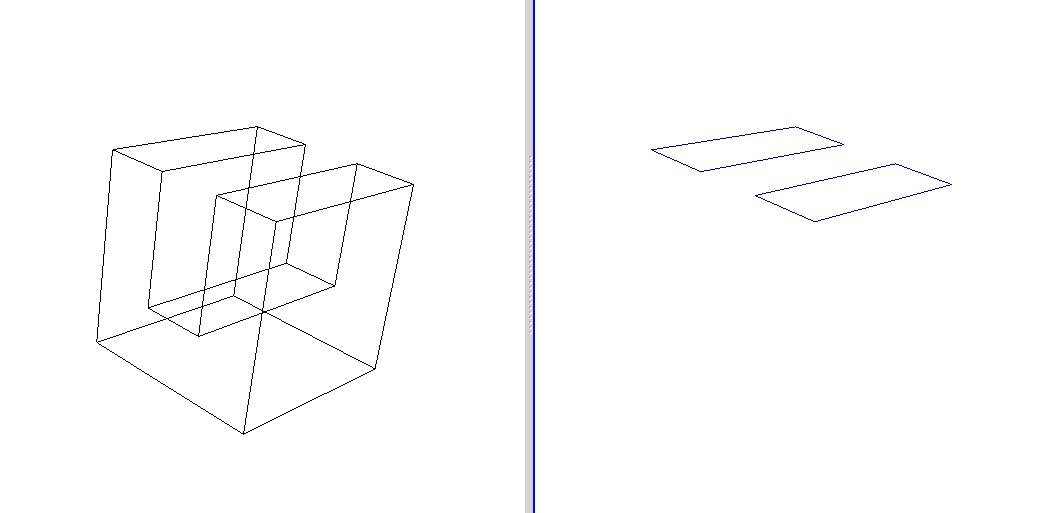
\includegraphics[width=15cm]{cube-cutted/cube-cutted-3.png}
		    \caption{Сечение многогранника cube-cutted плоскостью $z = 3$. Многогранник понимается как выпуклое
		замкнутое множество, поэтому считается, что грань, целиком лежащая в секущей плоскости,
		должна либо сама войти в новый многогранник, либо содержаться внутри какой-то новой грани.
		В приведенном выше примере две грани многогранника лежат в плоскости, а все остальные лежат
		ниже.}
		    \label{cube-cutted-3}
		\end{figure}
	\end{flushleft}

\newpage
\subsubsection{Тестирование на многограннике poly-big}
	\begin{flushleft}
		При тестировании возникают случаи, когда сечение имеет 2 или 3 компоненты
	\end{flushleft}
	\begin{flushleft}
		\begin{figure}[p]
		    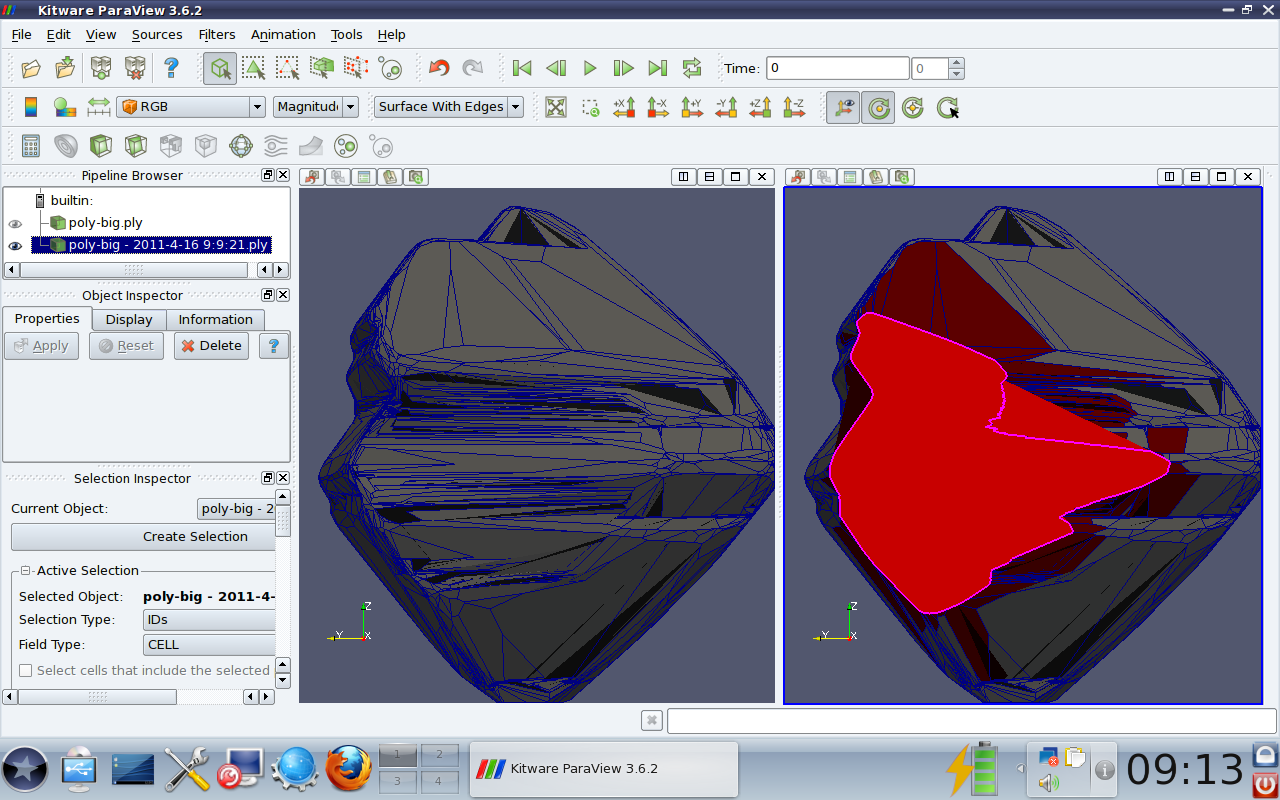
\includegraphics[trim = 220 65 10 140, clip, width=15cm]{poly-big/3.png}
		    \caption{Сечение многогранника poly-big плоскостью $x = -3$.}
		    \label{poly-big-1}
		\end{figure}
	\end{flushleft}
	\begin{flushleft}
		\begin{figure}[p]
		    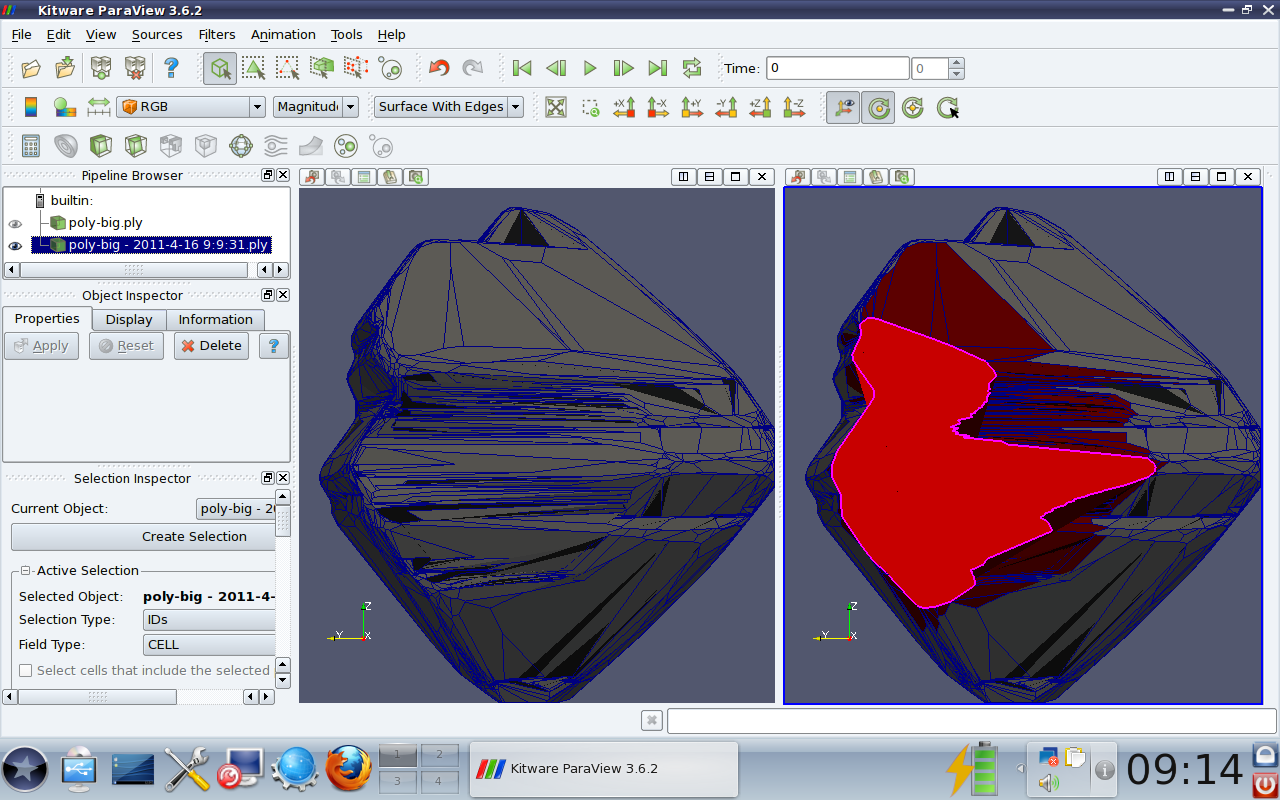
\includegraphics[trim = 220 65 10 140, clip, width=15cm]{poly-big/31.png}
		    \caption{Сечение многогранника poly-big плоскостью $x = -3.1$.}
		    \label{poly-big-2}
		\end{figure}
	\end{flushleft}
	\begin{flushleft}
		\begin{figure}[p]
		    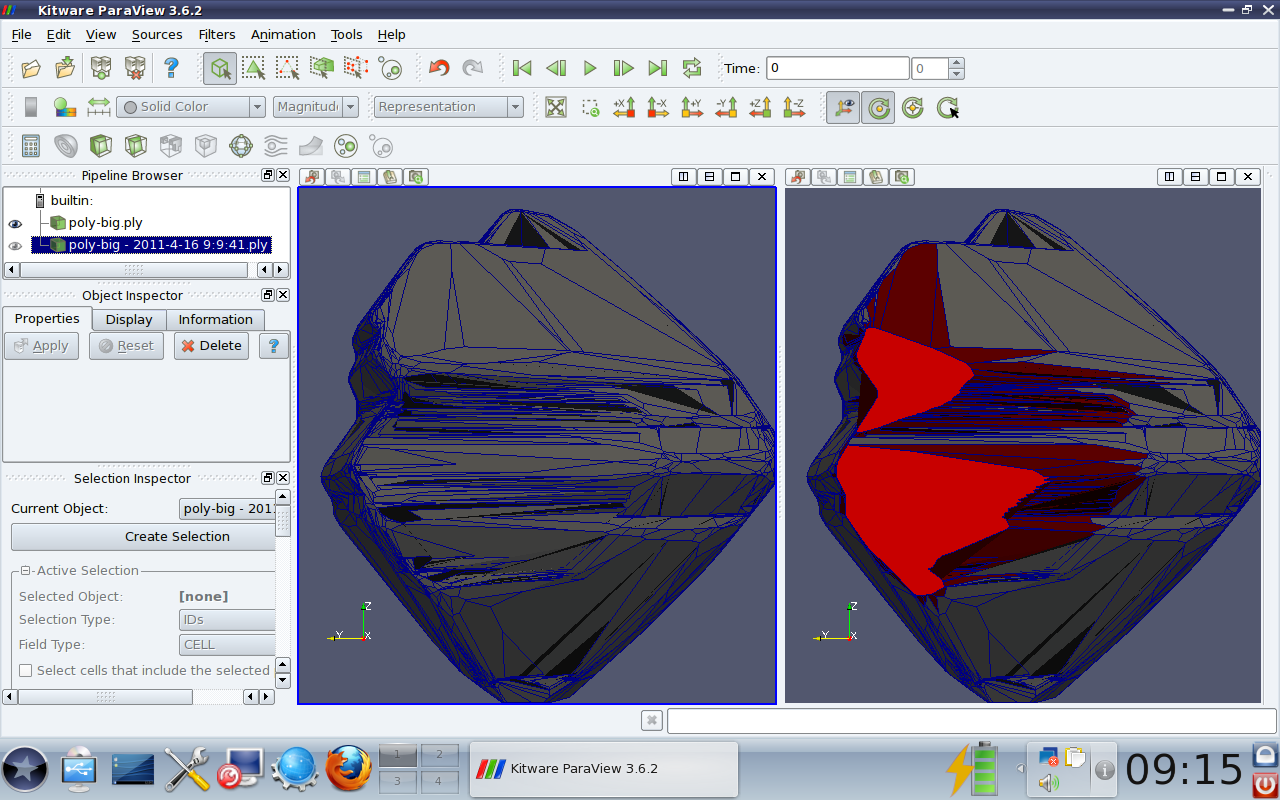
\includegraphics[trim = 220 65 10 140, clip, width=15cm]{poly-big/33.png}
		    \caption{Сечение многогранника poly-big плоскостью $x = -3.3$.}
		    \label{poly-big-3}
		\end{figure}

	\end{flushleft}
	\begin{flushleft}
		\begin{figure}[p]
		    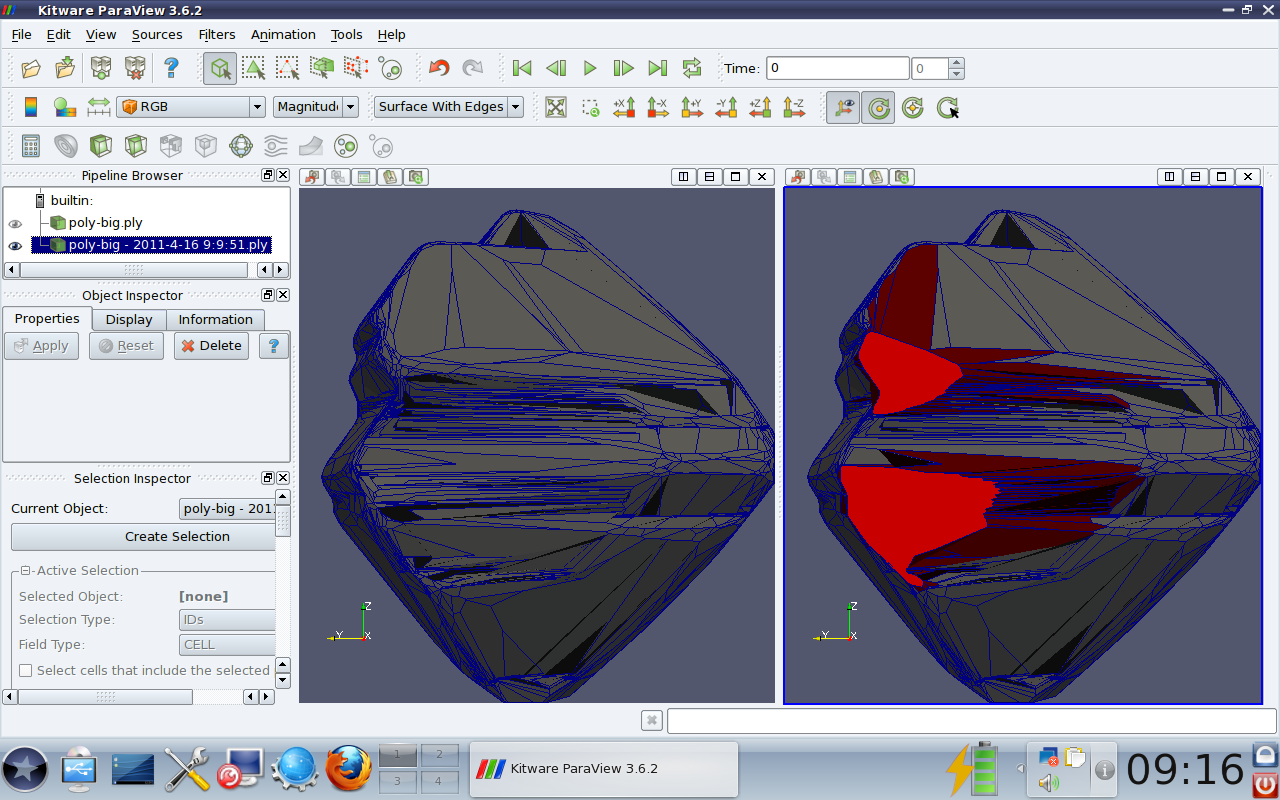
\includegraphics[trim = 220 65 10 140, clip, width=15cm]{poly-big/34.png}
		    \caption{Сечение многогранника poly-big плоскостью $x = -3.4$.}
		    \label{poly-big-4}
		\end{figure}
	\end{flushleft}
	\begin{flushleft}
		\begin{figure}[p]
		    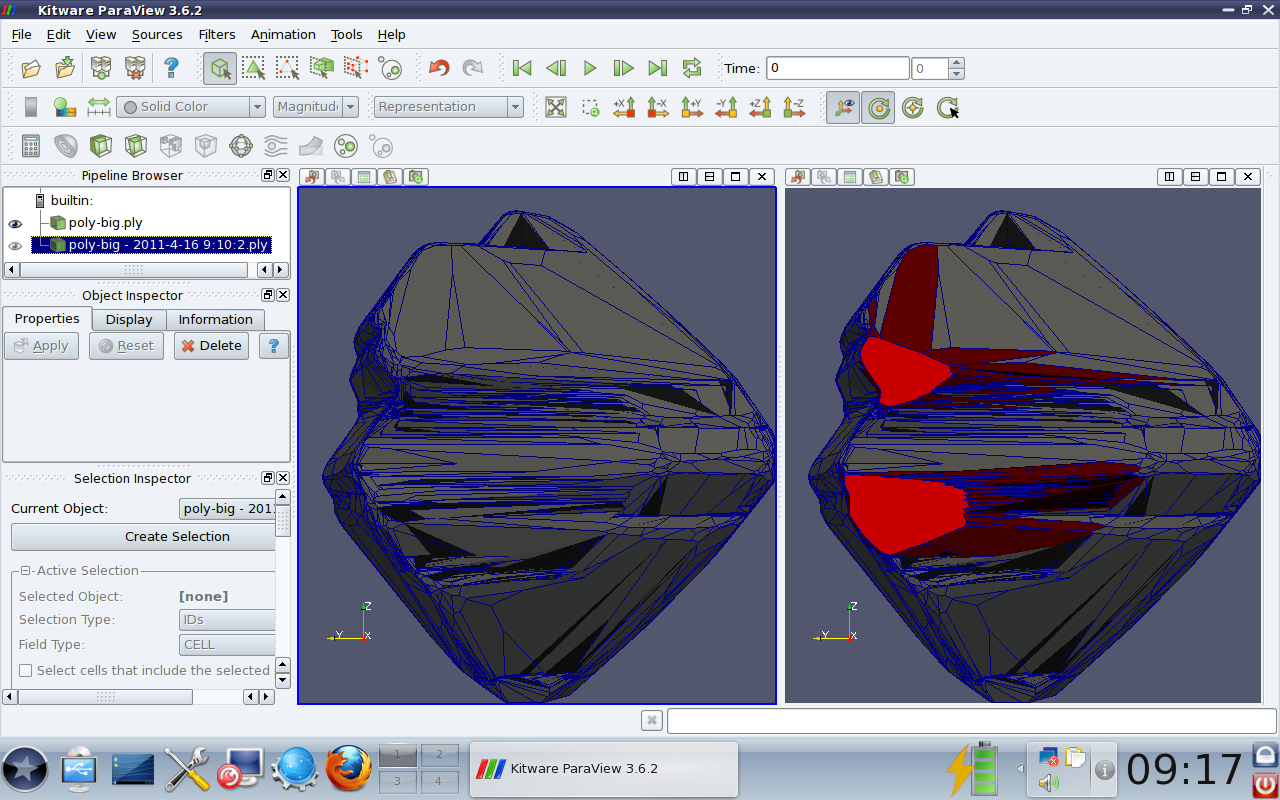
\includegraphics[trim = 220 65 10 140, clip, width=15cm]{poly-big/35.png}
		    \caption{Сечение многогранника poly-big плоскостью $x = -3.5$.}
		    \label{poly-big-5}
		\end{figure}

	\end{flushleft}
	\begin{flushleft}
		\begin{figure}[p]
		    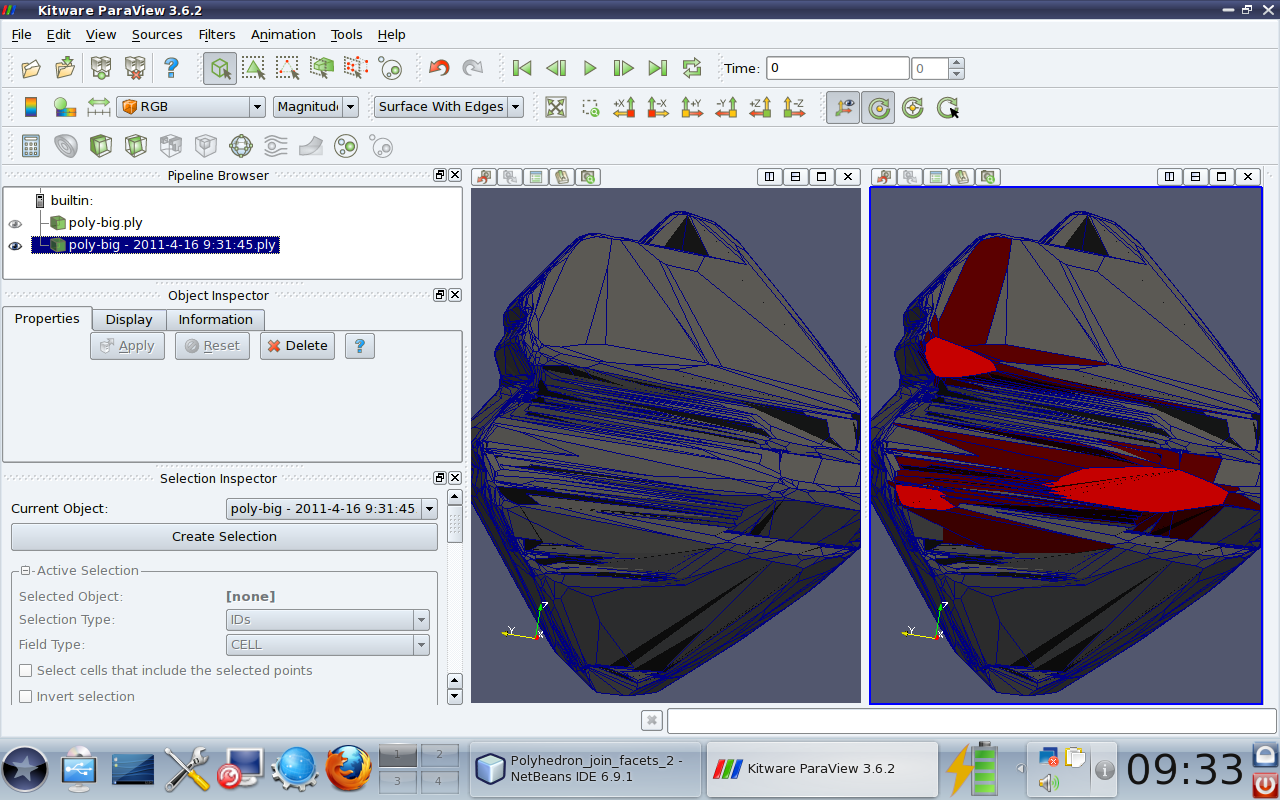
\includegraphics[trim = 350 65 10 140, clip, width=15cm]{poly-big/3components.png}
		    \caption{Сечение многогранника poly-big особой плоскостью, при котором образуется 3 компоненты в 
		    сечении.}
		    \label{poly-big-6}
		\end{figure}
	\end{flushleft}

\newpage
\subsection{Модификация алгоритма для задачи слияния смежных граней}

\begin{flushleft}
 В конце предыдущего раздела мы упомянули, что для того, чтобы применить программу рассечения многогранника в 
завершающем этапе алгоритма слияния граней, нужно ее немного модифицировать. Связано это с тем, что 
в многограннике, возникающем после поднятия вершин, лежащих ниже плоскости, может быть нарушена плоскостность
главной грани (т. е. той, которая является результатом слияния). Какие изменения нужно внести в алгоритм?
\end{flushleft}

\begin{flushleft}
 \textbf{1.} Сечение должно быть однокомпонентным, т. к. было бы бессмысленно в ответ на запрос слить две грани
выдавать в ответ две компоненты.
\end{flushleft}

\begin{flushleft}
 \textbf{2.} Главная грань, в которой нарушена плоскостность должна обрабатываться программой особым образом.
Для нее нужно построить список тех ее вершин, которые лежат в плоскости рассечения, причем в том порядке, в 
каком они встречаются в контуре (т. е. против часовой стрелки).
\end{flushleft}

\begin{flushleft}
 \textbf{3.} Начать строить контур нужно с грани, которая не является главной. Если в некоторый момент движения
произойдет выход на главную грань, то нужно просто последовательно собирать нужные точки грани. Чтобы при
этом не началось движение в обратную сторону, нужно с самого начала организовывать его против часовой стрелки.
\end{flushleft}




\newpage
\section{Подвижка вершины и дальнейшая перестройка многогранника}
\subsection{Идея задачи}
\begin{flushleft}
 В разделе "Введение" была сформулирована идея коррекции многогранника путем сглаживания граней. Она
возникла в результате анализа дефектов в процессе создания 3D-моделей реальных камней. Есть и другая
проблема, которая возникает в этом процессе. Дело в том, что как правило в многогранниках не бывает вершин
со степенью выше 3, а если в реальном камне таковые имеются, то они разбиваются на несколько вершин. 
Возникает ситуация, когда заведомо неоправданно увеличивается число точек и усложняется модель.
\end{flushleft}

\begin{flushleft}
  Как бороться с этой проблемой? Можно попытаться зарегистрировать такие "кучки" точек, заменять их на одну
вершину и затем перестраивать многогранник так, чтобы восстановилась плоскостность. Для начала, чтобы 
двигаться в этом направлении, нужно научиться менять местоположение хотя бы \textit{одной} точки. Итак,
возникает следующая задача.
\end{flushleft}

\begin{flushleft}
  Имеется многогранник, состоящий из вершин и граней. Все его точки с некоторой
погрешностью лежат в определенных гранях. Затем берется одна его точка,
меняется ее местоположение и фиксируется. \textbf{Требуется} скорректировать положение
точек и граней многогранника, чтобы точки вновь стали попадать в соответствующие
грани.
\end{flushleft}

\begin{flushleft}
  У этой задачи имеется несколько вариантов формализации.
\end{flushleft}

\subsection{Формализация задачи}
\subsubsection{Первый вариант: варьирование вершин}
	\begin{flushleft}
		Введем обозначения. Пусть вершины многогранника представлены следующим образом:
		$$
		  A^{0}_{1} = \begin{pmatrix}x^{0}_{1}\\y^{0}_{1}\\z^{0}_{1}\end{pmatrix},
		  A^{0}_{2} = \begin{pmatrix}x^{0}_{2}\\y^{0}_{2}\\z^{0}_{2}\end{pmatrix},
		  \ldots, 
		  A^{0}_{N} = \begin{pmatrix}x^{0}_{N}\\y^{0}_{N}\\z^{0}_{N}\end{pmatrix}.
		$$
		Пусть грани многогранника заданы следующим образом:
		$$\pi_{1} = A^{0}_{k(1, 1)} A^{0}_{k(1, 2)} \ldots A^{0}_{k(1, n_{1})},$$
		$$\pi_{2} = A^{0}_{k(2, 1)} A^{0}_{k(2, 2)} \ldots A^{0}_{k(2, n_{2})},$$
		$$\ldots$$
		$$\pi_{M} = A^{0}_{k(M, 1)} A^{0}_{k(M, 2)} \ldots A^{0}_{k(M, n_{M})}$$
		где $k(i, j)$ - $j$-я вершина в $i$-й грани, $n_{i}$ - количество вершин
		в $i$-й грани. $N$ - количество вершин многогранника, $M$ - количество граней
		многогранника
	\end{flushleft}
	\begin{flushleft}
		Деформируем $N$-ю точку многогранника: 
		$$
		  A_{N} = A^{0}_{N} + \Delta A_{N} = 
		  \begin{pmatrix}
				 x^{0}_{N} + \Delta x_{N}\\
				 y^{0}_{N} + \Delta y_{N}\\
				 z^{0}_{N} + \Delta z_{N}
		  \end{pmatrix},
		$$
		причем приращение $\Delta A_{N}$ фиксировано.
	\end{flushleft}
	\begin{flushleft}
		1). Вычислим для граней $\pi_{1}, \pi_{2}, \ldots, \pi_{M}$ те плоскости, в которых они
		реально расположены, - например, методом наименьших квадратов:
		$$\pi_{1} : a^{0}_{1} x + b^{0}_{1} y + c^{0}_{1} z + d^{0}_{1} = 0,$$
		$$\pi_{2} : a^{0}_{2} x + b^{0}_{2} y + c^{0}_{2} z + d^{0}_{2} = 0,$$
		$$\ldots$$
		$$\pi_{M} : a^{0}_{M} x + b^{0}_{M} y + c^{0}_{M} z + d^{0}_{M} = 0$$
		При расчете тех граней, к которым принадлежит подвинутая вершина $A_{N}$, нужно
		помнить, что точка должна лежать в этих гранях точно. Пусть таких граней всего $m_{N}$ 
		штук.
	\end{flushleft}
	\begin{flushleft}
		2). Решим следующую экстремальную задачу:
		$$
		  \sum\limits_{i = 1}^{N - 1}|\Delta A_{i}|^{2} = \sum\limits_{i = 1}^{N - 1}(|\Delta x_{i}|^{2} + |\Delta y_{i}|^{2} + |\Delta z_{i}|^{2}) = \to \min
		$$
		при следующих условиях связи:
		$$
			\left\{
				\begin{aligned}
					a^{0}_{1} x_{k(1, 1)} + b^{0}_{1} y_{k(1, 1)} + c^{0}_{1} z_{k(1, 1)} + d^{0}_{1} = 0 \\
					a^{0}_{1} x_{k(1, 2)} + b^{0}_{1} y_{k(1, 2)} + c^{0}_{1} z_{k(1, 2)} + d^{0}_{1} = 0 \\
					\ldots \\
					a^{0}_{1} x_{k(1, n_{1})} + b^{0}_{1} y_{k(1, n_{1})} + c^{0}_{1} z_{k(1, n_{1})} + d^{0}_{1} = 0 \\
					\ldots \\
					\ldots \\
					a^{0}_{m} x_{k(m, 1)} + b^{0}_{m} y_{k(m, 1)} + c^{0}_{m} z_{k(m, 1)} + d^{0}_{m} = 0 \\
					a^{0}_{m} x_{k(m, 2)} + b^{0}_{m} y_{k(m, 2)} + c^{0}_{m} z_{k(m, 2)} + d^{0}_{m} = 0 \\
					\ldots \\
					a^{0}_{m} x_{k(m, n_{m})} + b^{0}_{m} y_{k(m, n_{m})} + c^{0}_{m} z_{k(m, n_{m})} + d^{0}_{m} = 0
				\end{aligned}
			\right.
		$$
		Эти условия описывают тот факт, что вершины точным образом лежат на соответствующих им гранях.
		Число таких условий равно 
		$$
			\sum\limits_{i = 1}^{M}n_{i} - m_{N} = \sum\limits_{j = 1}^{N - 1}m_{j} \ge 3 (N - 1),
		$$
		поскольку каждая вершина лежит как минимум в трех гранях ($m_{j}$ - количество граней, содержащих $j$-ю
		вершину). Таким образом, мы имеем не менее $3 (N - 1)$ 
		условий относительно $3 (N - 1)$ переменных 
		$\Delta x_{i}, \Delta y_{i}, \Delta z_{i}, i = 1, \ldots, N - 1$. Если каждая вершина лежит ровно в трех 
		гранях, то для решения задачи нужно решить систему линейных уравнений методом Гаусса. Однако, ничего нельзя
		будет сказать о значении функционала на этом решении. В общем же случае система переопределена и решение
		найти нельзя. Есть несколько вариантов решить эту проблему.
	\end{flushleft}

\subsubsection{Второй вариант: варьирование вершин и граней}
	\begin{flushleft}
		Не будем фиксировать полученные уравнения плоскостей граней, т. е. введем в систему 
		дополнительные переменные
		$$
			\begin{aligned}
				a_{1} = a^{0}_{1} + \Delta a_{1}, 
				b_{1} = b^{0}_{1} + \Delta b_{1}, 
				c_{1} = c^{0}_{1} + \Delta c_{1}, 
				d_{1} = d^{0}_{1} + \Delta d_{1}, \\
				\ldots \\
				a_{1} = a^{0}_{M} + \Delta a_{M}, 
				b_{1} = b^{0}_{M} + \Delta b_{M}, 
				c_{1} = c^{0}_{M} + \Delta c_{M}, 
				d_{1} = d^{0}_{M} + \Delta d_{M}	
			\end{aligned}
		$$
		Рассмотрим тогда следующую экстремальную задачу
		$$	
			\sum\limits_{i = 1}^{N - 1}(|\Delta x_{i}|^{2} + |\Delta y_{i}|^{2} + |\Delta z_{i}|^{2}) + 
			\sum\limits_{j = 1}^{M}(|\Delta a_{j}|^{2} + |\Delta b_{j}|^{2} + |\Delta c_{j}|^{2} + 
			|\Delta d_{j}|^{2}) \to \min		
		$$
		при следующих условиях связи:
		$$
			\left\{
				\begin{aligned}
					a_{1} x_{k(1, 1)} + b_{1} y_{k(1, 1)} + c_{1} z_{k(1, 1)} + d_{1} = 0 \\
					a_{1} x_{k(1, 2)} + b_{1} y_{k(1, 2)} + c_{1} z_{k(1, 2)} + d_{1} = 0 \\
					\ldots \\
					a_{1} x_{k(1, n_{1})} + b_{1} y_{k(1, n_{1})} + c_{1} z_{k(1, n_{1})} + d_{1} = 0 \\
					\ldots \\
					\ldots \\
					a_{m} x_{k(m, 1)} + b_{m} y_{k(m, 1)} + c_{m} z_{k(m, 1)} + d_{m} = 0 \\
					a_{m} x_{k(m, 2)} + b_{m} y_{k(m, 2)} + c_{m} z_{k(m, 2)} + d_{m} = 0 \\
					\ldots \\
					a_{m} x_{k(m, n_{m})} + b_{m} y_{k(m, n_{m})} + c_{m} z_{k(m, n_{m})} + d_{m} = 0
				\end{aligned}
			\right.
		$$
		Поступим стандартным образом. Составим для этой задачи функцию Лагранжа:
		$$
			\begin{aligned}
				L = \sum\limits_{i = 1}^{N - 1}(|\Delta x_{i}|^{2} + |\Delta y_{i}|^{2} + |\Delta z_{i}|^{2})~ + ~\\
				~ + ~\sum\limits_{j = 1}^{M}(|\Delta a_{j}|^{2} + |\Delta b_{j}|^{2} + |\Delta c_{j}|^{2} + 
				|\Delta d_{j}|^{2})~ - ~\\
				~ - ~\sum\limits_{i = 1}^{M} \sum\limits_{j = 1} ^ {n_{i}} \lambda_{k(i, j)}
				(a_{i} x_{k(i, j)} + b_{i} y_{k(i, j)} + c_{i} z_{k(i, j)} + d_{i})		
			\end{aligned}
		$$
		Экстремум этой функции достигается в тех же точках, что и у исходного функционала. Продифференцируем эту
		фунцию и пририравняем частные производные к нулю:
$$
    \frac{\partial L}{\partial \Delta x_{1}} = 2 (x^{0}_{1} + \Delta x_{1}) - 
    \sum\limits_{\{i : A_{1} \in \pi_{i}\}} \lambda_{k(i, j_{i})} (a^{0}_{i} + \Delta a_{i}) = 0
$$
$$
    \frac{\partial L}{\partial \Delta y_{1}} = 2 (y^{0}_{1} + \Delta y_{1}) - 
    \sum\limits_{\{i : A_{1} \in \pi_{i}\}} \lambda_{k(i, j_{i})} (b^{0}_{i} + \Delta b_{i}) = 0
$$
$$
    \frac{\partial L}{\partial \Delta z_{1}} = 2 (z^{0}_{1} + \Delta z_{1}) - 
    \sum\limits_{\{i : A_{1} \in \pi_{i}\}} \lambda_{k(i, j_{i})} (c^{0}_{i} + \Delta c_{i}) = 0
$$
$$
    \ldots
$$
$$
    \frac{\partial L}{\partial \Delta x_{N - 1}} = 2 (x^{0}_{N - 1} + \Delta x_{N - 1}) - 
    \sum\limits_{\{i : A_{N - 1} \in \pi_{i}\}} \lambda_{k(i, j_{i})} (a^{0}_{i} + \Delta a_{i}) = 0
$$
$$
    \frac{\partial L}{\partial \Delta y_{N - 1}} = 2 (y^{0}_{N - 1} + \Delta y_{N - 1}) - 
    \sum\limits_{\{i : A_{N - 1} \in \pi_{i}\}} \lambda_{k(i, j_{i})} (b^{0}_{i} + \Delta b_{i}) = 0
$$
$$
    \frac{\partial L}{\partial \Delta z_{N - 1}} = 2 (z^{0}_{N - 1} + \Delta z_{N - 1}) - 
    \sum\limits_{\{i : A_{N - 1} \in \pi_{i}\}} \lambda_{k(i, j_{i})} (c^{0}_{i} + \Delta c_{i}) = 0
$$
$$
    \frac{\partial L}{\partial \Delta a_{1}} = 2 (a^{0}_{1} + \Delta a_{1}) - 
    \sum\limits_{j = 1}^{n_{1}} \lambda_{k(1, j)} (x^{0}_{k(1, j)} + \Delta x_{k(1, j)}) = 0
$$
$$
    \frac{\partial L}{\partial \Delta b_{1}} = 2 (b^{0}_{1} + \Delta b_{1}) - 
    \sum\limits_{j = 1}^{n_{1}} \lambda_{k(1, j)} (y^{0}_{k(1, j)} + \Delta y_{k(1, j)}) = 0
$$
$$
    \frac{\partial L}{\partial \Delta c_{1}} = 2 (c^{0}_{1} + \Delta c_{1}) - 
    \sum\limits_{j = 1}^{n_{1}} \lambda_{k(1, j)} (z^{0}_{k(1, j)} + \Delta z_{k(1, j)}) = 0
$$
$$
    \frac{\partial L}{\partial \Delta d_{1}} = 2 (d^{0}_{1} + \Delta d_{1}) - 
    \sum\limits_{j = 1}^{n_{1}} \lambda_{k(1, j)} = 0
$$
$$
    \ldots
$$
$$
    \frac{\partial L}{\partial \Delta a_{M}} = 2 (a^{0}_{M} + \Delta a_{M}) - 
    \sum\limits_{j = 1}^{n_{M}} \lambda_{k(M, j)} (x^{0}_{k(M, j)} + \Delta x_{k(M, j)}) = 0
$$
$$
    \frac{\partial L}{\partial \Delta b_{M}} = 2 (b^{0}_{M} + \Delta b_{M}) - 
    \sum\limits_{j = 1}^{n_{M}} \lambda_{k(M, j)} (y^{0}_{k(M, j)} + \Delta y_{k(M, j)}) = 0
$$
$$
    \frac{\partial L}{\partial \Delta c_{M}} = 2 (c^{0}_{M} + \Delta c_{M}) - 
    \sum\limits_{j = 1}^{n_{M}} \lambda_{k(M, j)} (z^{0}_{k(M, j)} + \Delta z_{k(M, j)}) = 0
$$
$$
    \frac{\partial L}{\partial \Delta d_{M}} = 2 (d^{0}_{M} + \Delta d_{M}) - 
    \sum\limits_{j = 1}^{n_{M}} \lambda_{k(M, j)} = 0
$$
		Вместе с условиями связи эти равенства образуют систему из 
		$3 (N - 1) + 4 M + \sum\limits_{i = 1}^{M}n_{i} - m_{N}$ уравнений относительно
		$3 (N - 1) + 4 M + \sum\limits_{i = 1}^{M}n_{i} - m_{N}$ неизвестных. Решение этой системы нелинейных
		уравнений представляет собой открытый вопрос.
	\end{flushleft}	




\subsubsection{Третий вариант: поочередное варьирование вершин и граней}
\begin{flushleft}
Здесь же вариация происходит поочередно:\\
	\textbf{1. }Вычисляем плоскости методом наименьших квадратов\\
	\textbf{2. }Изменяем координаты вершин таким образом, чтобы минимизировать функционал\\
$$	
	J = \sum\limits_{i = 1}^{N - 1}(|x_{i} - x_{i}^{0}|^{2} + |y_{i} - y_{i}^{0}|^{2} 
	+ |z_{i} - z_{i}^{0}|^{2}) + 
	K\sum\limits_{j = 1}^{M}\sum\limits_{i: A_{i} \in \pi_{j}}
	|a_{j}x_{i} + b_{j}y_{i} + c_{j}z_{i} + d_{j}|^{2} \to \min		
$$
При этом нужно помнить, что коэффициенты уравнений плоскостей на этом шаге уже фиксированы, и менять
их не нужно. Переменная $K$ называется штрафом\\
	\textbf{3. }Возвращаемся к пункту 1. и т. д.\\
\end{flushleft}

\begin{flushleft}
 Решим задачу минимизации функционала $J$. Запишем частные производные функционала по переменным 
$x_{i}, y_{i}, z_{i}$ и приравняем их к нулю.
\end{flushleft}

\begin{flushleft}
$$
  \frac{\partial J}{\partial x_{i}} = 2 x_{i} - 2 x_{i}^{0} + 
  2 K \sum\limits_{j: A_{i} \in \pi_{j}}
  a_{j} (a_{j}x_{i} + b_{j}y_{i} + c_{j}z_{i} + d_{j}) = 0
$$
$$
  \frac{\partial J}{\partial y_{i}} = 2 y_{i} - 2 y_{i}^{0} + 
  2 K \sum\limits_{j: A_{i} \in \pi_{j}}
  b_{j} (a_{j}x_{i} + b_{j}y_{i} + c_{j}z_{i} + d_{j}) = 0
$$
$$
  \frac{\partial J}{\partial z_{i}} = 2 z_{i} - 2 z_{i}^{0} + 
  2 K \sum\limits_{j: A_{i} \in \pi_{j}}
  c_{j} (a_{j}x_{i} + b_{j}y_{i} + c_{j}z_{i} + d_{j}) = 0
$$
\end{flushleft}
\begin{flushleft}
 Заметим, что система расщепляется на системы размерности 3x3. В матричной форме они будут иметь
вид:
$$
  \begin{pmatrix}
    1 + K (a, a) & (a, b) & (a, c)\\
    (a, b) & 1 + K (b, b) & (b, c)\\
    (a, c) & (b, c) & 1 + K (c, c)
  \end{pmatrix}
  \begin{pmatrix}
    x_{i}\\
    y_{i}\\
    z_{i}
  \end{pmatrix} = 
  \begin{pmatrix}
    -K (a, d) + x_{i}^{0}\\
    -K (b, d) + y_{i}^{0}\\
    -K (c, d) + z_{i}^{0}
  \end{pmatrix}
$$
\end{flushleft}
\begin{flushleft}
 Здесь введены такие обозначения: $(a, a) = \sum\limits_{j: A_{i} \in \pi_{j}}a_{j}^{2}$,
$(a, a) = \sum\limits_{j: A_{i} \in \pi_{j}}a_{j}^{2}$,
$(b, b) = \sum\limits_{j: A_{i} \in \pi_{j}}b_{j}^{2}$,
$(c, c) = \sum\limits_{j: A_{i} \in \pi_{j}}c_{j}^{2}$,
$(a, b) = \sum\limits_{j: A_{i} \in \pi_{j}}a_{j}b_{j}$,
$(a, c) = \sum\limits_{j: A_{i} \in \pi_{j}}a_{j}c_{j}$,
$(b, c) = \sum\limits_{j: A_{i} \in \pi_{j}}b_{j}c_{j}$,
$(a, d) = \sum\limits_{j: A_{i} \in \pi_{j}}a_{j}d_{j}$,
$(b, d) = \sum\limits_{j: A_{i} \in \pi_{j}}b_{j}d_{j}$,
$(c, d) = \sum\limits_{j: A_{i} \in \pi_{j}}c_{j}d_{j}$.
\end{flushleft}

\begin{flushleft}
 Данные обозначения можно интерпретировать еще и как скалярные произведения векторов $a$, 
$b$, $c$, $d$ - записанных в строку коэффициентов тех граней, в которых содержится точка $A_{i}$.
\end{flushleft}

\begin{flushleft}
 Имеет ли эта система решение? Представим ее матрицу в следующем виде:
 $$
  \begin{pmatrix}
    1 + K (a, a) & (a, b) & (a, c)\\
    (a, b) & 1 + K (b, b) & (b, c)\\
    (a, c) & (b, c) & 1 + K (c, c)
  \end{pmatrix} = 
  \begin{pmatrix}
    1 & 0 & 0\\
    0 & 1 & 0\\
    0 & 0 & 1\\
  \end{pmatrix} + K
  \begin{pmatrix}
    (a, a) & (a, b) & (a, c)\\
    (a, b) & (b, b) & (b, c)\\
    (a, c) & (b, c) & (c, c)
  \end{pmatrix}
$$
Таким образом, матрица представляется в виде суммы единичной матрицы и матрицы Грама векторов
$a$, $b$, $c$, которая является положительно определенной. Значит и исходная матрица положительно
определена, более того, она симметрична, значит система невырождена и обязательно имеет решение.
\end{flushleft}

\subsection{Тестирование алгоритма}
\begin{flushleft}
Выше представлен всего лишь примерный план реализации алгоритма. В действительности есть много его модификаций: от
тех, которые дают довольно адекватный результат, до тех, которые полностью "выворачивают" многогранник 
наизнанку. При этом происходят следующие процессы: в гранях (как в многоугольниках) возникают 
самопересечения, некоторые ребра начинают пересекать те грани, в которых они не лежат.
\end{flushleft}
\begin{flushleft}
Множественность возникает из-за того, что задаче есть два изменяемых параметра:\\
	\textbf{1. }Штраф $K$. Каким его сделать? Если слишком большим, то алгоритм перестанет 
"чувствовать" смещения вершин, а если слишком малым, то наооброт - алгоритм будет плохо решать задачу
восстановления плоскостности многогранника.\\
	\textbf{2. }Как чередовать шаги 1 и 2? Менять ли при этом штраф $K$?\\
\end{flushleft}

\subsubsection{Экспоненциальный рост штрафа, локальная минимизация}
\begin{flushleft}
 В результате тестирования одним из приемлемых оказался следующий подход. Минимизируется не функционал
$$
	J = \sum\limits_{i = 1}^{N - 1}(|x_{i} - x_{i}^{0}|^{2} + |y_{i} - y_{i}^{0}|^{2} 
	+ |z_{i} - z_{i}^{0}|^{2}) + 
	K\sum\limits_{j = 1}^{M}\sum\limits_{i: A_{i} \in \pi_{j}}
	|a_{j}x_{i} + b_{j}y_{i} + c_{j}z_{i} + d_{j}|^{2},
$$ но функционал
$$
  \begin{aligned}
	J = \sum\limits_{i = 1}^{N - 1}(|x_{i}^{(n+1)} - x_{i}^{(n)}|^{2} + |y_{i}^{(n+1)} - y_{i}^{(n)}|^{2} 
	+ |z_{i}^{(n+1)} - z_{i}^{(n)}|^{2}) + \\
	+ K\sum\limits_{j = 1}^{M}\sum\limits_{i: A_{i} \in \pi_{j}}
	|a_{j}x_{i}^{(n+1)} + b_{j}y_{i}^{(n+1)} + c_{j}z_{i}^{(n+1)} + d_{j}|^{2},
  \end{aligned}
$$то есть минимизируется не сдвиг в целом, а лишь сдвиг на каждом шаге. При этом не обязательно находится
минимум исходного функционала, а лишь некоторая конфигурация многогранника, которая удовлетворяет условиям
плоскостности, не являясь, вообще говоря, оптимальной.
\end{flushleft}
\begin{flushleft}
Следующий алгоритм позволил достичь удовлетворительных результатов:\\
\end{flushleft}
\begin{flushleft}
$K = 100$\\
$\varepsilon = 10^{-7}$\\
Цикл. Делать 10 раз:\\
\verb"{"\\
\quadДелать: \\
\quad\verb"{"\\
\quad\quadВычислить новые плоскости методом наименьших квадратов\\
\quad\quadВычислить координаты вершин, минимизирующих функционал со штрафом, равным $K$\\
\quad\quadВычислить погрешность попадания вершин в плоскости\\
\quad\verb"}"пока (эта погрешность больше, чем $\varepsilon$)\\
\quadУвеличиваем $K$ в два раза\\
\quadУменьшаем $\varepsilon$ в два раза\\
\verb"}"\\
\end{flushleft}

\begin{flushleft}
Как этот алгоритм работает? На тестируемых многогранниках он выдал следующее поведение. Программа заходит в цикл 1, затем в нем - 
в цикл 2, делает примерно 30 шагов, выходит из 2 цикла, снова начинает 2 цикл (с увеличенным в 2 раза штрафом и с уменьшенной в 
2 раза погрешностью), но теперь уже делает только 1 шаг, снова выходит из 2 цикла и т. д. - всего примерно 10 раз.
Вот таблица результатов алгоритма ($\Delta$ - сумарный сдвиг вершин, $\varepsilon$ - погрешность попадания вершин в плоскости,
$\varepsilon_{0}$ - граница погрешности, пересечение которой обеспечивает конец цикла 2, $K$ - штраф):\\
\begin{tabular}{|c|c|c|c|c|c|}
\hline
 цикл 1 & цикл 2 & $\Delta$ & $\varepsilon$& $\varepsilon_{0}$&  $K$\\
\hline
 0 & 0 & 0.114942 & 4.220043e-02 & 1.000000e-07 & 100.000000\\
\hline
 0 & 1 & 0.048647 & 2.640706e-02 & 1.000000e-07 & 100.000000\\
\hline
 0 & 2 & 0.018739 & 1.637491e-02 & 1.000000e-07 & 100.000000\\
\hline
 0 & 3 & 0.007239 & 1.015491e-02 & 1.000000e-07 & 100.000000\\
\hline
 0 & 4 & 0.002856 & 6.344031e-03 & 1.000000e-07 & 100.000000\\
\hline
 0 & 5 & 0.001151 & 3.991388e-03 & 1.000000e-07 & 100.000000\\
\hline
 0 & 6 & 0.000472 & 2.528785e-03 & 1.000000e-07 & 100.000000\\
\hline
 0 & 7 & 0.000196 & 1.634950e-03 & 1.000000e-07 & 100.000000\\
\hline
 0 & 8 & 0.000082 & 1.064094e-03 & 1.000000e-07 & 100.000000\\
\hline
 0 & 9 & 0.000035 & 6.940496e-04 & 1.000000e-07 & 100.000000\\
\hline
 0 & 10 & 0.000015 & 4.535194e-04 & 1.000000e-07 & 100.000000\\
\hline
 0 & 11 & 0.000006 & 2.967911e-04 & 1.000000e-07 & 100.000000\\
\hline
 0 & 12 & 0.000003 & 1.944614e-04 & 1.000000e-07 & 100.000000\\
\hline
 0 & 13 & 0.000001 & 1.275375e-04 & 1.000000e-07 & 100.000000\\
\hline
 0 & 14 & 0.000001 & 8.370982e-05 & 1.000000e-07 & 100.000000\\
\hline
 0 & 15 & 0.000000 & 5.497753e-05 & 1.000000e-07 & 100.000000\\
\hline
 0 & 16 & 0.000000 & 3.612497e-05 & 1.000000e-07 & 100.000000\\
\hline
 0 & 17 & 0.000000 & 2.374594e-05 & 1.000000e-07 & 100.000000\\
\hline
 0 & 18 & 0.000000 & 1.561315e-05 & 1.000000e-07 & 100.000000\\
\hline
 0 & 19 & 0.000000 & 1.026795e-05 & 1.000000e-07 & 100.000000\\
\hline
 0 & 20 & 0.000000 & 6.753804e-06 & 1.000000e-07 & 100.000000\\
\hline
 0 & 21 & 0.000000 & 4.442928e-06 & 1.000000e-07 & 100.000000\\
\hline
 0 & 22 & 0.000000 & 2.923018e-06 & 1.000000e-07 & 100.000000\\
\hline
 0 & 23 & 0.000000 & 1.923204e-06 & 1.000000e-07 & 100.000000\\
\hline
 0 & 24 & 0.000000 & 1.265446e-06 & 1.000000e-07 & 100.000000\\
\hline
 0 & 25 & 0.000000 & 8.326840e-07 & 1.000000e-07 & 100.000000\\
\hline
 0 & 26 & 0.000000 & 5.479375e-07 & 1.000000e-07 & 100.000000\\
\hline
 0 & 27 & 0.000000 & 3.605724e-07 & 1.000000e-07 & 100.000000\\
\hline
 0 & 28 & 0.000000 & 2.372805e-07 & 1.000000e-07 & 100.000000\\
\hline
 0 & 29 & 0.000000 & 1.561485e-07 & 1.000000e-07 & 100.000000\\
\hline
 0 & 30 & 0.000000 & 1.027587e-07 & 1.000000e-07 & 100.000000\\
\hline
 0 & 31 & 0.000000 & 6.762423e-08 & 1.000000e-07 & 100.000000\\
\hline
 1 & 32 & 0.000000 & 2.585086e-08 & 5.000000e-08 & 200.000000\\
\hline
 2 & 33 & 0.000000 & 9.229164e-09 & 2.500000e-08 & 400.000000\\
\hline
 3 & 34 & 0.000000 & 3.159339e-09 & 1.250000e-08 & 800.000000\\
\hline
 4 & 35 & 0.000000 & 1.053913e-09 & 6.250000e-09 & 1600.000000\\
\hline
 5 & 36 & 0.000000 & 3.462331e-10 & 3.125000e-09 & 3200.000000\\
\hline
 6 & 37 & 0.000000 & 1.131674e-10 & 1.562500e-09 & 6400.000000\\
\hline
 7 & 38 & 0.000000 & 3.720410e-11 & 7.812500e-10 & 12800.000000\\
\hline
 8 & 39 & 0.000000 & 1.253741e-11 & 3.906250e-10 & 25600.000000\\
\hline
 9 & 40 & 0.000000 & 4.448228e-12 & 1.953125e-10 & 51200.000000\\
\hline
\end{tabular}
\end{flushleft}

\subsubsection{Масштабирование штрафа, локальная минимизация}
\begin{flushleft}
 Можно попробовать реализовать следующую идею.
\end{flushleft}
\begin{flushleft}
$$	
	J(x) = \sum\limits_{i = 1}^{N - 1}(|\Delta x_{i}|^{2} + |\Delta y_{i}|^{2} + |\Delta z_{i}|^{2}) + 
	K\sum\limits_{j = 1}^{M}\sum\limits_{i: A_{i} \in \pi_{j}}
	|a_{j}x_{i} + b_{j}y_{i} + c_{j}z_{i} + d_{j}|^{2}  = 
	S_{1} + K S_{2}
$$
Пусть теперь $S_{1} = \varepsilon_{1}$, $S_{2} = \varepsilon_{2}$.\\
Тогда выберем $K = \frac{\varepsilon_{1}}{\varepsilon_{2}}$.\\
Это дает преимущество в том, что теперь слагаемые будут одного порядка.
\end{flushleft}
\begin{flushleft}
 Прежний алгоритм выдавал вот такие результаты: 
\end{flushleft}

\begin{flushleft}
\begin{tabular}{|p{1cm}|p{1cm}|p{4cm}|p{4cm}|p{3cm}|}

\hline 
 цикл 1 & цикл 2 & $S_{2}$, погрешности попаданий в плоскости & $S_{1}$, сдвиги вершин& штраф $K$ \\
\hline
 0 & 0 & 4.509368e-03 & 1.224731e-03 & 100.000000\\
\hline
 0 & 1 & 2.818460e-03 & 1.055994e-03 & 100.000000\\
\hline
 \dots & \dots & \dots & \dots & \dots\\
\hline
 0 & 10 & 5.619919e-05 & 1.414728e-03 & 100.000000\\
\hline
 \dots & \dots & \dots & \dots & \dots\\
\hline
 0 & 27 & 7.088412e-08 & 1.435461e-03 & 100.000000\\
\hline
 1 & 28 & 2.768007e-08 & 1.435470e-03 & 200.000000\\
\hline
 2 & 29 & 1.009637e-08 & 1.435476e-03 & 400.000000\\
\hline
 3 & 30 & 3.540058e-09 & 1.435479e-03 & 800.000000\\
\hline
 4 & 31 & 1.210947e-09 & 1.435482e-03 & 1600.000000\\
\hline
 5 & 32 & 4.084458e-10 & 1.435484e-03 & 3200.000000\\
\hline
 6 & 33 & 1.370517e-10 & 1.435485e-03 & 6400.000000\\
\hline
 7 & 34 & 4.614675e-11 & 1.435486e-03 & 12800.000000\\
\hline
 8 & 35 & 1.591248e-11 & 1.435486e-03 & 25600.000000\\
\hline
 9 & 36 & 5.662650e-12 & \textbf{1.435487e-03} & 51200.000000\\
\hline
\end{tabular}
\end{flushleft}

\begin{flushleft}
 Новый алгоритм выдал такие результаты
\end{flushleft}

\begin{flushleft}
 \begin{tabular}{|p{1cm}|p{5cm}|p{4cm}|p{3cm}|}
\hline
цикл & $S_{2}$, погрешности попаданий в плоскости & $S_{1}$, сдвиги вершин& штраф $K$ \\
  \hline
 0 & 3.517835e-02 & 1.615489e-05 & 0.392949\\
\hline
 100 & 4.049939e-02 & 8.219693e-06 & 0.000203\\
\hline
 \dots & \dots & \dots & \dots\\
\hline
 2000 & 5.218465e-03 & 6.583846e-04 & 0.123768\\
\hline
 2059 & 3.083940e-04 & 7.281009e-04 & 1.975172\\
\hline
 2060 & 2.520618e-04 & 7.286694e-04 & 2.360944\\
\hline
 2061 & 1.999617e-04 & 7.291923e-04 & 2.890836\\
\hline
 2062 & 1.527278e-04 & 7.296639e-04 & 3.646660\\
\hline
 2063 & 1.112085e-04 & 7.300783e-04 & 4.777544\\
\hline
 2064 & 7.646352e-05 & 7.304289e-04 & 6.564948\\
\hline
 2065 & 4.911293e-05 & 7.307096e-04 & 9.552645\\
\hline
 2066 & 2.932750e-05 & 7.309185e-04 & 14.878152\\
\hline
 2067 & 1.642868e-05 & 7.310611e-04 & 24.922635\\
\hline
 2068 & 8.918421e-06 & 7.311513e-04 & 44.499065\\
\hline
 2069 & 4.825920e-06 & 7.312062e-04 & 81.982142\\
\hline
 2070 & 2.578748e-06 & 7.312397e-04 & 151.516422\\
\hline
 2071 & 1.301561e-06 & 7.312606e-04 & 283.563904\\
\hline
 2072 & 5.751982e-07 & 7.312737e-04 & 561.833444\\
\hline
 2073 & 1.913991e-07 & 7.312819e-04 & 1271.342200\\
\hline
 2074 & 3.378585e-08 & 7.312870e-04 & 3820.717979\\
\hline
 2075 & 1.477041e-09 & 7.312901e-04 & 21644.771524\\
\hline
 2076 & 7.527428e-12 & \textbf{7.312920e-04} & 495104.846438\\
\hline
 \end{tabular}
\end{flushleft}
\begin{flushleft}
 Вывод: ценой увеличения числа шагов в 50 раз получили выигрыш: фунционал
$$	
	S_{1}(x) = \sum\limits_{i = 1}^{N - 1}(|\Delta x_{i}|^{2} + |\Delta y_{i}|^{2} + |\Delta z_{i}|^{2})\to \min		
$$
уменьшается в 2 раза, то есть от 1.435487e-03 до 7.312920e-04
\end{flushleft}

\begin{flushleft}
Недостатки у данного алгоритма следующие:\\
 	\textbf{1. }Нет гарантий сходимости алгоритма\\
	\textbf{2. }Алгоритм работает слишком долго (слишком много шагов)\\
	\textbf{3. }Часто алгоритм вообще расходится\\
\end{flushleft}

\subsubsection{Экспоненциальный рост штрафа, глобальная минимизация}
\begin{flushleft}
  Были произведены попытки тестирования также и минимизации отклонения в целом, то есть функионала
$$
	J = \sum\limits_{i = 1}^{N - 1}(|x_{i} - x_{i}^{0}|^{2} + |y_{i} - y_{i}^{0}|^{2} 
	+ |z_{i} - z_{i}^{0}|^{2}) + 
	K\sum\limits_{j = 1}^{M}\sum\limits_{i: A_{i} \in \pi_{j}}
	|a_{j}x_{i} + b_{j}y_{i} + c_{j}z_{i} + d_{j}|^{2},
$$
При этом оказалось, что метод масштабирования для данного функционала не работает (по крайней мере на
рассмотренном примере). Приемлемые результаты позволил достичь следующий алгоритм:
\end{flushleft}

\begin{flushleft}
$K = 100$\\
$\varepsilon = $погрешности попадания вершин в плоскости\\
%$\varepsilon = 10^{-7}$\\
%Цикл. Делать 10 раз:\\
Пока ($\varepsilon > 10^{-10}$)\\
\verb"{"\\
\quadВычислить новые плоскости методом наименьших квадратов\\
\quadВычислить координаты вершин, минимизирующих функционал со штрафом, равным $K$\\
%\quadВычислить погрешность попадания вершин в плоскости\\
\quadУвеличиваем $K$ в 2 раза\\
\quad$\varepsilon = $погрешности попадания вершин в плоскости\\
%\quadУменьшаем $\varepsilon$ в 2 раза\\
\verb"}"\\
\end{flushleft}

\begin{flushleft}
Этот алгоритм демонстрирует следующее поведение:\\
\begin{tabular}{|p{1cm}|p{1cm}|p{4cm}|p{4cm}|p{3cm}|}

\hline 
 цикл 1 & цикл 2 & $S_{2}$, погрешности попаданий в плоскости & $S_{1}$, сдвиги вершин& штраф $K$ \\

\hline
 0 & 0 & 1.846692e-02 & 2.614818e-04 & 100.000000\\
\hline
 \ldots & \ldots & \ldots & \ldots & \ldots \\
%\hline
% 10 & 10 & 1.920185e-04 & 1.409526e-03 & 102400.000000\\
%\hline
% \ldots & \ldots & \ldots & \ldots & \ldots \\
%\hline
% 20 & 20 & 3.206267e-06 & 1.429711e-03 & 104857600.000000\\
%\hline
% \ldots & \ldots & \ldots & \ldots & \ldots \\
%\hline
% 30 & 30 & 5.661824e-08 & 1.430056e-03 & 107374182400.000000\\
%\hline
% \ldots & \ldots & \ldots & \ldots & \ldots \\
% 40 & 40 & 1.005028e-09 & 1.430062e-03 & 109951162777600.000000\\
%\hline
% \ldots & \ldots & \ldots & \ldots & \ldots \\
\hline
 46 & 46 & 8.992944e-11 & \textbf{1.430062e-03} & 7e15\\
\hline
\end{tabular}
\end{flushleft}

\begin{flushleft}
Если же в алгоритме $K$ увеличивать, а $\varepsilon$ уменьшать не в 2, а в 1,005 раза,
то результаты будут более точными:\\
\begin{tabular}{|p{1cm}|p{1cm}|p{4cm}|p{4cm}|p{3cm}|}

\hline 
 цикл 1 & цикл 2 & $S_{2}$, погрешности попаданий в плоскости & $S_{1}$, сдвиги вершин& штраф $K$ \\

\hline
 0 & 0 & 1.846692e-02 & 2.614818e-04 & 100.000000\\
\hline
 \ldots & \ldots & \ldots & \ldots & \ldots \\
\hline
 3433 & 3433 & 9.964233e-11 & \textbf{7.339104e-04} & 2e9\\
\hline
\end{tabular}
\end{flushleft}

\begin{flushleft}
 Таким образом, замедление алгоритма в 100 раз позволяет уменьшить функционал
$$	
	S_{1}(x) = \sum\limits_{i = 1}^{N - 1}(|\Delta x_{i}|^{2} + |\Delta y_{i}|^{2} + |\Delta z_{i}|^{2})\to \min		
$$
всего в 2 раза, т. е. от 1.430062e-03 до 7.339104e-04.
\end{flushleft}


\subsubsection{Сбор статистики о выворачивании}
\begin{flushleft}
 Статистика собиралась следующим образом. Для каждого многогранника 100 раз случайным образом
выбиралась вершина. Затем для этой вершины вычислялось расстояние $\delta$ от нее до ближайшей вершины.
После этого случайным образом вабиралось направление (три случайных числа) и оно нормировалось так, чтобы
длина этого вектора была равна $\delta$, $0.5\delta$, $0.1\delta$, $0.05\delta$, $0.01\delta$, $0.005\delta$, $0.001\delta$,
$0.0005\delta$, $0.0001\delta$, или $0.00005\delta$. \\
Производилась деформация. Если после этого многогранник выворачивался или если алгоритм не давал
результата за нужное число шагов, то этот факт регистрировался.\\
Так делалось для каждой из 100 случайно выбранных вершин многогранника.
\end{flushleft}

\begin{flushleft}
Имя многогранника: poly-small\\
\begin{tabular}{|c|c|}
\hline
	Порядок сдвига & Вероятность "выворачивания"\\
\hline
	1.000000 &	0.770000\\
\hline
	0.500000 &	0.530000\\
\hline
	0.100000 &	0.360000\\
\hline
	0.050000 &	0.230000\\
\hline
	0.010000 &	0.090000\\
\hline
	0.005000 &	0.060000\\
\hline
	0.001000 &	0.000000\\
\hline
	0.000500 &	0.000000\\
\hline
	0.000100 &	0.000000\\
\hline
	0.000050 &	0.000000\\
\hline
\end{tabular} 
\end{flushleft}

\begin{flushleft}
Имя многогранника: poly-med\\
\begin{tabular}{|c|c|}
\hline
	Порядок сдвига & Вероятность "выворачивания"\\
\hline
	1.000000 &	0.720000\\
\hline
	0.500000 &	0.600000\\
\hline
	0.100000 &	0.210000\\
\hline
	0.050000 &	0.150000\\
\hline
	0.010000 &	0.040000\\
\hline
	0.005000 &	0.020000\\
\hline
	0.001000 &	0.010000\\
\hline
	0.000500 &	0.010000\\
\hline
	0.000100 &	0.000000\\
\hline
	0.000050 &	0.010000\\
\hline
\end{tabular}
\end{flushleft}

\begin{flushleft}
Имя многогранника: polyhedron-2010-11-25\\
\begin{tabular}{|c|c|}
\hline
	Порядок сдвига & Вероятность "выворачивания"\\
\hline
	1.000000 &	0.810000\\
\hline
	0.500000 &	0.740000\\
\hline
	0.100000 &	0.280000\\
\hline
	0.050000 &	0.240000\\
\hline
	0.010000 &	0.090000\\
\hline
	0.005000 &	0.000000\\
\hline
	0.001000 &	0.010000\\
\hline
	0.000500 &	0.000000\\
\hline
	0.000100 &	0.000000\\
\hline
	0.000050 &	0.000000\\
\hline
\end{tabular}
\end{flushleft}

\begin{flushleft}
Имя многогранника: polyhedron-2010-12-19\\
\begin{tabular}{|c|c|}
\hline
	Порядок сдвига & Вероятность "выворачивания"\\
\hline
	1.000000 &	0.790000\\
\hline
	0.500000 &	0.660000\\
\hline
	0.100000 &	0.190000\\
\hline
	0.050000 &	0.120000\\
\hline
	0.010000 &	0.000000\\
\hline
	0.005000 &	0.000000\\
\hline
	0.001000 &	0.000000\\
\hline
	0.000500 &	0.000000\\
\hline
	0.000100 &	0.000000\\
\hline
	0.000050 &	0.000000\\
\hline
\end{tabular}
\end{flushleft}

\begin{flushleft}
 \textbf{Вывод. }Чтобы гарантировать корректность многогранника, нужно брать деформацию на 2-3 порядка меньше, чем 
расстояние до ближайшего соседа.
\end{flushleft}

\subsubsection{Регистрирование выворачиваний}
\begin{flushleft}
 Представляют интерес следующие вопросы:\\
\textbf{1.} В какой момент, то есть на каком шаге происходит выворачивание?\\
\textbf{2.} Что при этом происходит, то есть почему нарушается корректность многогранника?\\
\textbf{3.} Как бороться с выворачиванием? Возможно поменять топологическую структуру многогранника так,
чтобы можно было ликвидировать выворачивания?
\end{flushleft}

\begin{flushleft}
 Был протестирован многогранник "poly-small"  из 48 вершин и 26 граней, у которого 3-я вершина сдвигалась 
на вектор (-0.1, 0.1, 0.1), имеющий длину, большую, чем минимальное расстояние от этой вершины до 
других вершин. Следующая таблица показывает, на каких шагах алгоритма возникали самопересечения.
\end{flushleft}

\begin{flushleft}
 \begin{tabular}{|p{1cm}|p{3cm}|p{3cm}|p{3cm}|p{3cm}|}
  \hline
  Номер шага & $S_{2}$, погрешности попаданий в плоскости & $S_{1}$, сдвиги вершин& штраф $K$ & 
  Число самопересечений\\
  \hline
  189 & 1.244817e-01 & 4.667703e-02 & 0.344241 & 1\\
  \hline
  193 & 9.534896e-02 & 5.219574e-02 & 0.495032 & 2\\
  \hline
  197 & 6.643063e-02 & 5.753278e-02 & 0.764622 & 3\\
  \hline
  198 & 5.948548e-02 & 5.878811e-02 & 0.866058 & 4\\
  \hline
 \end{tabular}
\end{flushleft}

\begin{flushleft}
 На рис. ~\ref{consections-1}, ~\ref{consections-2}, ~\ref{consections-3} и ~\ref{consections-4} 
показаны 4 последовательные самопересечения, которые были зарегистрированы. Нужно заметить, что
если самопересечение возникало на каком-то шаге, то оно сохранялось и дальше, более того, оно 
еще более усугублялось.
\end{flushleft}


\begin{flushleft}
  \begin{figure}[h]
    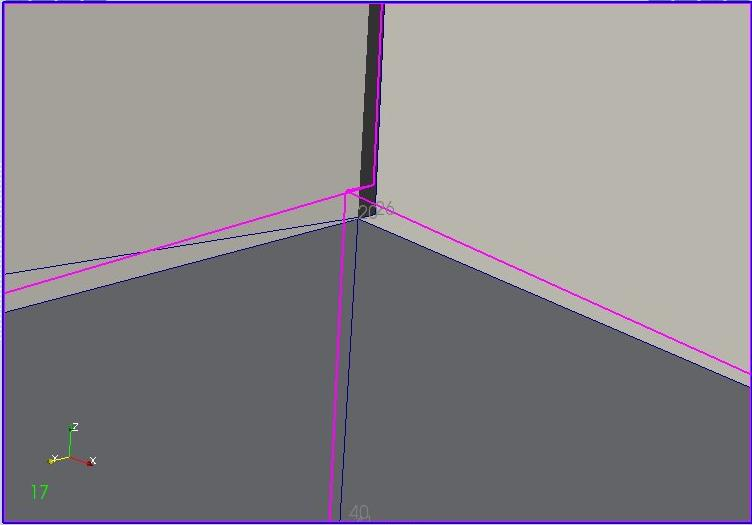
\includegraphics[clip, width=13cm]{img/consections-1.jpeg}
    \caption{Первое зарегистрированное самопересечение}\label{consections-1}
  \end{figure}
\end{flushleft}
\begin{flushleft}
  \begin{figure}[h]
    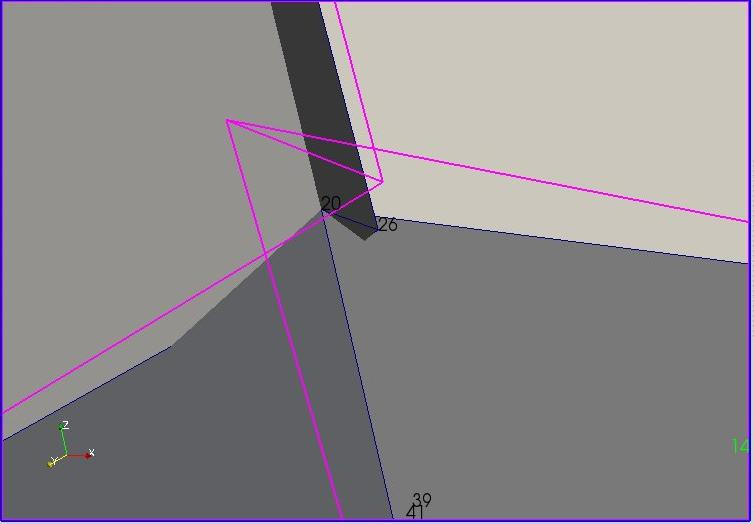
\includegraphics[clip, width=13cm]{img/consections-2.jpeg}
    \caption{Второе зарегистрированное самопересечение}\label{consections-2}
  \end{figure}
\end{flushleft}
\begin{flushleft}
  \begin{figure}[h]
    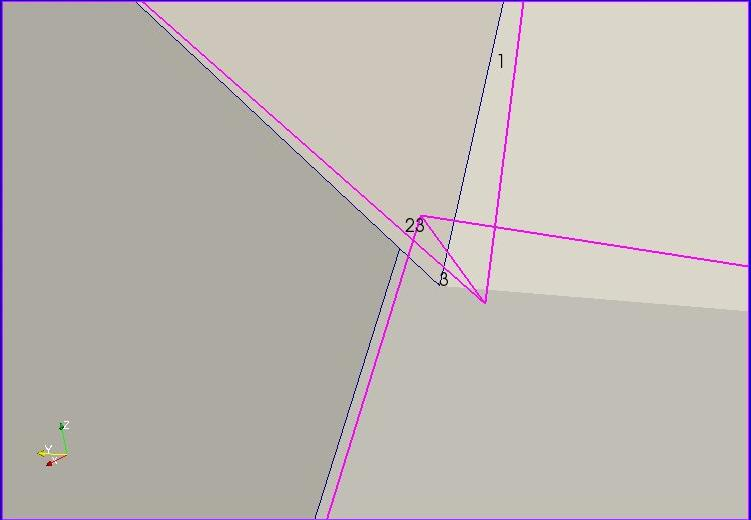
\includegraphics[clip, width=13cm]{img/consections-3.jpeg}
    \caption{Третье зарегистрированное самопересечение}\label{consections-3}
  \end{figure}
\end{flushleft}
\begin{flushleft}
  \begin{figure}[h]
    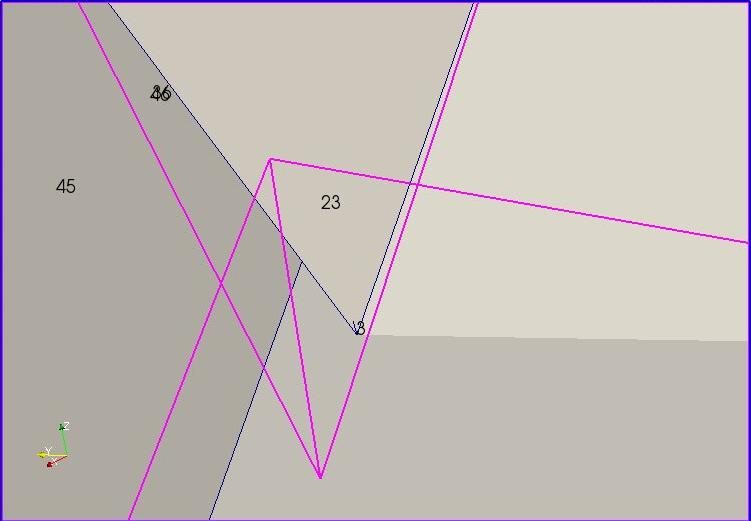
\includegraphics[clip, width=13cm]{img/consections-4.jpeg}
    \caption{Четвертое зарегистрированное самопересечение}\label{consections-4}
  \end{figure}
\end{flushleft}
\begin{flushleft}
  \begin{figure}[h]
    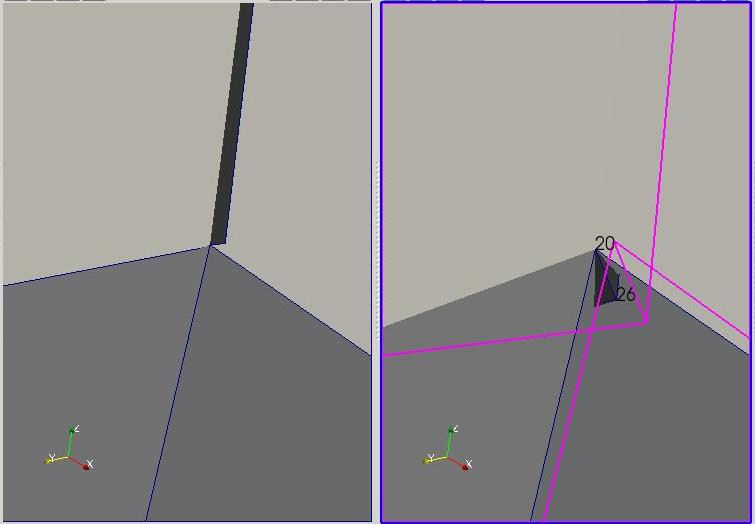
\includegraphics[clip, width=13cm]{img/consections-5.jpeg}
    \caption{С течением времени самопересечение усугубляется}\label{consections-5}
  \end{figure}
\end{flushleft}





\subsubsection{TODO: Устранение выворачиваний путем слияния вершин}

%Нужно реализовать следующие идеи:\\
%	\textbf{1. }Попробовать разную динамику изменения штрафа. Не только 
%экспоненциальный рост, но и линейный, логарифмический...\\
%	\textbf{2. }Решить проблему ``выворачивания'' многогранника. Дело в том, что если 
%начальная деформация точки слишком велика, то нарушается корректность многогранника 
%(грани выворачиваются или наезжают друг на друга). В продемонстрированном выше примере точка двигалась
%на расстояние порядка 0.1, тогда как одно из ребер, из нее исходящих, имеет длину порядка 0.03. 
%Вот что при этом наблюдается:\\
%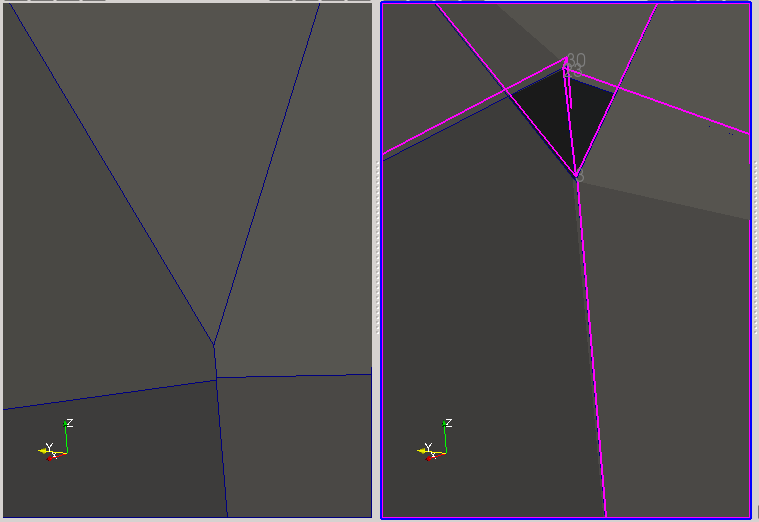
\includegraphics[clip, width=15cm]{img/2-1.png}
%При решении проблемы выворачнивания нужно решить, вообще говоря, три задачи:\\
%	\textbf{2.1. }На какое максимальное расстояние расстояние можно двигать точку, не изменяя при этом топологической структуры 
%многогранника?\\
%	\textbf{2.2. }Попытаться делать деформацию не разом за одно применение программы, а, скажем, делить вектор сдвига на 10 частей
%и за 10 применений программы реализовать сдвиг.\\
%	\textbf{2.3. }Если эти две задачи решены, то может быть попытаться решить задачу, когда сдвиг больше допустимого, то есть когда
%мы сначала сдвигаем точку на максимально допустимое расстояние, затем меняем немного структуру многогранника, а затем сдвигаем еще раз.
%(???)

\subsection{TODO: Анализ сходимости и трудоемкости алгоритма}
Про сходимость алгоритма до сих пор ничего не известно, доказать не удалось.
(TODO)

\newpage
\section{Заключение}

\newpage
\begin{thebibliography}{99}                    % Список литературы
\addcontentsline{toc}{section}{Список литературы}

\bibitem{wiki-ogranka}
http://ru.wikipedia.org/wiki/Огранка

\bibitem{3dbook}
http://3dbook.octonus.com/data/3dbook.html

\bibitem{wiki-almaz}
http://ru.wikipedia.org/wiki/Алмаз

\bibitem{doc-1}
OctoNus Software Ltd, Документация программы Helium Rough and Pacor 
(http://www.octonus.com/oct/support/doc/scanning.html)

\bibitem{doc-2}
OctoNus Software Ltd, Helium Polish - system for scanning of diamonds, документация, стр. 42
(http://www.octonus.com/oct/download/files/Helium\_system\_manual.pdf)

\end{thebibliography}

\end{document}



